\documentclass[11pt,a4paper]{article}

% ── Packages ──────────────────────────────────────────────────────────────
\usepackage[margin=1in]{geometry}
\usepackage{graphicx}
\usepackage{subcaption}
\usepackage{booktabs}
\usepackage{multirow}
\usepackage[table]{xcolor}
\usepackage{hyperref}
\usepackage{amsmath,amssymb}
\usepackage{enumitem}
\usepackage[font=small,labelfont=bf]{caption}
\usepackage{natbib}
\usepackage[capitalise,noabbrev]{cleveref}

% ── Path shortcuts ────────────────────────────────────────────────────────
\graphicspath{
  {../../results/}
  {../../../../references/Anthropic_paper_md/images/}
}

% ── Colors ────────────────────────────────────────────────────────────────
\definecolor{passgreen}{HTML}{2E7D32}
\definecolor{failred}{HTML}{C62828}
\definecolor{nomatch}{HTML}{FDDEDE}    % light red — intentional difference
\definecolor{unspecified}{HTML}{FFF3CD} % light yellow — absent from paper
\newcommand{\pass}{\textcolor{passgreen}{\textbf{PASS}}}
\newcommand{\fail}{\textcolor{failred}{\textbf{FAIL}}}

% ══════════════════════════════════════════════════════════════════════════
\title{Reproduction Report (Part 1): Identifying and Validating Emotion Vectors\\
       \large Llama 3.1 8B Instruct --- v2 Full-Scale (171 Emotions)}
\author{Junyuan Hong\\
  Mass General Hospital \& Harvard Medical School\\
  \texttt{jhong28@mgh.harvard.edu}}
\date{April 2026}

\begin{document}
\maketitle

% ══════════════════════════════════════════════════════════════════════════
\begin{abstract}
We independently reproduce and extend Part~1 of ``Emotion Concepts and
their Function in a Large Language Model''
\citep{anthropic2025emotion}, replacing the original closed-weight
Claude Sonnet~4.5 with the open-weight Llama~3.1~8B~Instruct
\citep{llama31}.  Our reproduction confirms that the core phenomena ---
\emph{emotion vector} formation (extracting linear directions in hidden
states that correspond to specific emotions), implicit emotion
detection, numerical modulation, and emotion-preference correlation ---
generalize to a
smaller, independently trained model, with \textbf{10 of 11}
verification criteria passing.  The causal steering correlation
($r{=}0.955$) closely matches the original ($r{=}0.85$), confirming
that emotion vectors causally influence model preferences across model
families.  The only failing criterion (V11: sign consistency, 25/35
vs.\ threshold 25) passes at the boundary.  We provide a
side-by-side comparison of every figure and metric, document
implementation choices for details absent from the original paper, and
release all code and data.
\end{abstract}

% ══════════════════════════════════════════════════════════════════════════
\section{Introduction}

Recent work by \citet{anthropic2025emotion}
presents compelling evidence that Claude Sonnet~4.5 forms robust
internal representations of emotion concepts --- linear directions in
the model's \emph{residual stream} (the sequence of hidden-state
vectors passed between transformer layers) that activate in
semantically appropriate contexts, predict the model's self-reported
preferences, and causally influence its behavior when used for
\emph{activation steering} (adding a direction vector to the hidden
states during inference to shift model behavior).  These findings have
significant implications for mechanistic interpretability and AI safety,
as they suggest that large language models develop structured
\emph{affective} representations --- i.e., representations encoding
emotional valence (positive vs.\ negative affect) and arousal --- that
play a functional role in downstream behavior.

However, two limitations hinder follow-up research.  First, \textbf{the
original implementation is not publicly available}: the paper describes
the methodology at a high level but does not release code, requiring
independent reimplementation to build upon or extend the results.
Second, \textbf{the study is conducted exclusively on Claude
Sonnet~4.5}, a large closed-weight model whose architecture and
parameter count are undisclosed.  It remains unclear whether the
reported phenomena --- emotion vector formation, implicit detection,
preference correlation, and causal steering --- are specific to this
particular model family and scale, or whether they generalize to
smaller, open-weight models with different training procedures and
safety alignment strategies.

This work addresses both limitations.  We present a full-scale,
independent reproduction of Part~1 using Llama~3.1~8B~Instruct \citep{llama31}, a
publicly available 8-billion-parameter model.\footnote{An earlier v1
reproduction used 30 emotions, 10 topics, and 5 stories/topic.  The
v2 methodology reported here addresses those scale limitations and
matches the original paper's full configuration.}  Our contributions
are:
\begin{enumerate}[nosep]
  \item \textbf{Open reimplementation.}  We implement the complete
        experimental pipeline --- from story generation and activation
        extraction through logit lens analysis (projecting internal
        vectors through the model's output vocabulary matrix to inspect
        which tokens they promote), implicit detection, numerical
        modulation, preference correlation, and causal steering ---
        guided by the published methodology, with
        Claude~Code (powered by Claude Opus~4.6) as the development
        agent prompted by the authors.
        All code, data, and analysis scripts are available for
        inspection and extension.
  \item \textbf{Cross-model comparison.}  We perform a systematic
        side-by-side comparison of every figure and metric between the
        original (Claude Sonnet~4.5) and our reproduction
        (Llama~3.1~8B), identifying which conclusions from Part~1
        generalize, which require qualification, and what model-specific
        behavioral differences emerge --- particularly in the causal
        steering regime where safety alignment interacts with emotion
        vector interventions.
\end{enumerate}

In summary, our reproduction achieves 10 of 11 verification criteria
(V1--V10, plus V11 at the boundary), with V11 (sign consistency: 25/35
vs.\ threshold $\geq$25) as the only narrow pass.  The strongest results are in implicit
detection (V3: 9/12, V4: 1.33), numerical modulation (V5: 19/24, V6:
19/24), and emotion-preference correlation (V9: 137/171 emotions with
$|r|>0.3$, where $r$ denotes the Pearson correlation coefficient
measuring linear association between two variables).  The causal
steering correlation $r=0.955$ closely matches the original's $r=0.85$,
confirming robust causal structure.  Several implementation details absent from
the original paper (Elo rating parameters, steered/control activity
split, steering token span, steering layer count) were filled with
reasonable
defaults and are documented in Table~\ref{tab:methods}.

% ══════════════════════════════════════════════════════════════════════════
% \clearpage
\section{Methods}

Table~\ref{tab:methods} provides a side-by-side comparison of every
design choice between the original paper and our reproduction.  We
match the original methodology wherever specified and document our
choices where details are absent.

\begin{table}[htbp]
  \centering
  \caption{\textbf{Methodology comparison: Original paper vs.\
  reproduction.}
  \colorbox{nomatch}{\strut Light red} = intentional difference;
  \colorbox{unspecified}{\strut Light yellow} = absent from the paper
  ($\dagger$), filled with our own choice.}
  \label{tab:methods}
  \small
  \begin{tabular}{p{3.4cm}p{4.4cm}p{4.4cm}c}
    \toprule
    \textbf{Design choice} & \textbf{Original (Anthropic)}
      & \textbf{Reproduction (ours)} & \textbf{Match?} \\
    \midrule
    \multicolumn{4}{l}{\emph{Model}} \\
    \rowcolor{nomatch}
    Architecture
      & Claude Sonnet~4.5 (closed)
      & \textbf{Llama~3.1 8B Instruct (open)} & No \\
    \rowcolor{unspecified}
    Parameters
      & Not disclosed
      & 8B & --- \\
    \rowcolor{unspecified}
    Layers / $d_{\text{model}}$ (hidden dim.)
      & Not disclosed
      & 32 / 4096 & --- \\
    \midrule
    \multicolumn{4}{l}{\emph{Data generation}} \\
    Emotions
      & 171 & 171 & Yes \\
    Topics
      & 100 & 100 & Yes \\
    Stories / topic / emotion
      & 12 & 12 & Yes \\
    Total stories
      & 205{,}200 & 205{,}200 & Yes \\
    Story length
      & $\sim$1 paragraph & $\sim$100--150 words & Yes \\
    Emotion word filter
      & Yes (stories avoid naming the emotion) & Yes & Yes \\
    \rowcolor{unspecified}
    Neutral transcripts
      & ``A set'' (count not specified)$^\dagger$
      & 200 factual Q\&A dialogues & --- \\
    \midrule
    \multicolumn{4}{l}{\emph{Vector extraction}} \\
    Activation pooling
      & Mean from token~50 onward & Mean from token~50 onward & Yes \\
    Vector computation
      & Per-emotion mean $-$ global mean & Same & Yes \\
    Confound removal
      & PCA (principal component analysis) on neutral acts, 50\% var.\ threshold & Same & Yes \\
    Analysis layer
      & ``$\approx$2/3 through the model''
      & Layer~21 of 32 ($= 0.66$) & Yes \\
    \midrule
    \multicolumn{4}{l}{\emph{Validation}} \\
    Logit lens (V1--V2)
      & Top-$k$ tokens via unembed & Same ($k{=}20$) & Yes \\
    Implicit detection (V3--V4)
      & 12 scenarios, cosine similarity & Same & Yes \\
    Numerical modulation (V5--V6)
      & 6 templates, 4 emotions each & Same & Yes \\
    Activity categories
      & 8 categories, 64 activities & Same activities & Yes \\
    Preference query format
      & ``Would you prefer (A) or (B)?'' & Same & Yes \\
    \rowcolor{unspecified}
    Elo $K$ factor
      & Not specified$^\dagger$ & $K = 32$ & --- \\
    \rowcolor{unspecified}
    Elo iterations
      & Not specified$^\dagger$ & 10 (early stop) & --- \\
    Steered/control split
      & Two equal groups (odd-indexed = steered)
      & Odd-indexed = steered within each category & Yes \\
    Steering strength
      & $0.5 \times \bar{\|h\|}$ & Same & Yes \\
    \rowcolor{unspecified}
    Steering layer(s)
      & ``Same middle layers''$^\dagger$
      & Single layer~21 & --- \\
    \rowcolor{unspecified}
    Steering token span
      & ``Token positions of steered activities''$^\dagger$
      & Character-to-token mapping & --- \\
    Steered emotions
      & 35 & 35 (top by $|r|$ from V9) & Yes \\
    \bottomrule
  \end{tabular}
\end{table}

\paragraph{Discussion of differences.}
The only intentional difference is the model: we use Llama~3.1~8B
Instruct (open-weight, 8B parameters) instead of Claude Sonnet~4.5
(closed-weight, undisclosed size).  This is the core question of the
reproduction: do emotion vector phenomena generalize across model
families?  All other design choices match the paper where specified.

For the six details marked $\dagger$ (absent from the paper), our
choices follow standard practices: the Elo rating system
(Section~\ref{sec:v7}) uses $K{=}32$ and 10 iterations as common
defaults; the steered/control split is stratified by category
for balance; steering is applied at the single analysis layer (the
paper's ``same middle layers'' may imply multiple layers, which could
affect steering magnitude); and the token span is identified by
approximate character-to-token mapping.  The most impactful absent
detail is likely the Elo parameters, which directly affect the Elo
range and therefore the steering $\Delta$ magnitude
(Section~\ref{sec:delta-scale}).

\paragraph{Implementation environment.}
All experiments were implemented using Claude~Code powered by
Claude~Opus~4.6 \citep{anthropic2025claude} as the development agent,
prompted by the authors.  The target model
(Llama~3.1~8B~Instruct, float16) was run on $2\times$~NVIDIA~A30 GPUs.
Story generation ($\sim$205{,}200 stories) took $\sim$16 hours using
batched multi-prompt inference (batch size 450) with automatic OOM
recovery.

% ══════════════════════════════════════════════════════════════════════════
\section{Results}

% ── 3.1  Logit Lens ──────────────────────────────────────────────────────
\subsection{Logit Lens (V1, V2)}

\paragraph{Method.}
The logit lens projects each emotion vector through the model's
unembedding matrix $W_{\text{unembed}}$ to identify which output tokens
each vector promotes or suppresses.  For each emotion $e$ with
unit-normalized vector $\hat{v}_e$ at the analysis layer, we compute
$\ell = W_{\text{unembed}} \cdot \hat{v}_e \in \mathbb{R}^{|\mathcal{V}|}$,
where $|\mathcal{V}|$ is the vocabulary size.  The top-$k$ entries of
$\ell$ reveal which tokens the emotion vector upweights (positive) or
downweights (negative) in the output distribution.

\textbf{V1 (self-recognition):} For each of the 171 emotions, we check
whether the emotion's own token ID (obtained via
\texttt{tokenizer.encode(emotion)}) appears among the top-20 token IDs
ranked by $\ell$.

\textbf{V2 (cross-valence):} For 5 opposite-valence pairs
(happy/sad, calm/desperate, proud/ashamed, excited/bored,
loving/hostile), we compute the dot product of their logit-space
vectors.  A negative dot product confirms that the two emotions push the
output distribution in opposing directions.

\paragraph{Results.}
\textbf{V1 --- Self-recognition: 57/171} (\pass, need $\geq$20).
33\% of emotions have their exact token ID in the top-20.\footnote{An
earlier version reported 9/171 due to a tokenizer mismatch: the check
used \texttt{tokenizer.encode("excited")} (no leading space) but the
logit lens top-20 contained space-prefixed tokens
(\texttt{" excited"}).  Including both variants fixed the count.}

\textbf{V2 --- Cross-valence: 5/5} (\pass).
All opposite-valence pairs have negative dot products.

% \clearpage
% ── 3.2  Implicit Detection ──────────────────────────────────────────────
\subsection{Implicit Emotion Detection (V3, V4)}

\paragraph{Method.}
We construct 12 short scenarios that imply specific emotions without
naming them (e.g., ``My daughter just took her first steps today!'' for
happy; ``My dog passed away'' for sad).  Each scenario is fed to the
model and the residual stream activation at the last token is extracted
at the analysis layer.  We then compute the cosine similarity between
each scenario's activation and each of the 12 corresponding emotion
vectors, producing a $12 \times 12$ matrix.

\textbf{V3 (diagonal dominance):} Count how many of the 12 scenarios
have their intended emotion as the argmax (highest cosine similarity)
across all 12 probes.

\textbf{V4 (mean diagonal rank):} For each scenario, rank the 12
probes by cosine similarity and record the rank of the intended emotion.
V4 is the mean of these ranks (1.0 = perfect).

\paragraph{Results.}

\begin{figure}[htbp]
  \centering
  \begin{subfigure}[t]{0.48\textwidth}
    \centering
    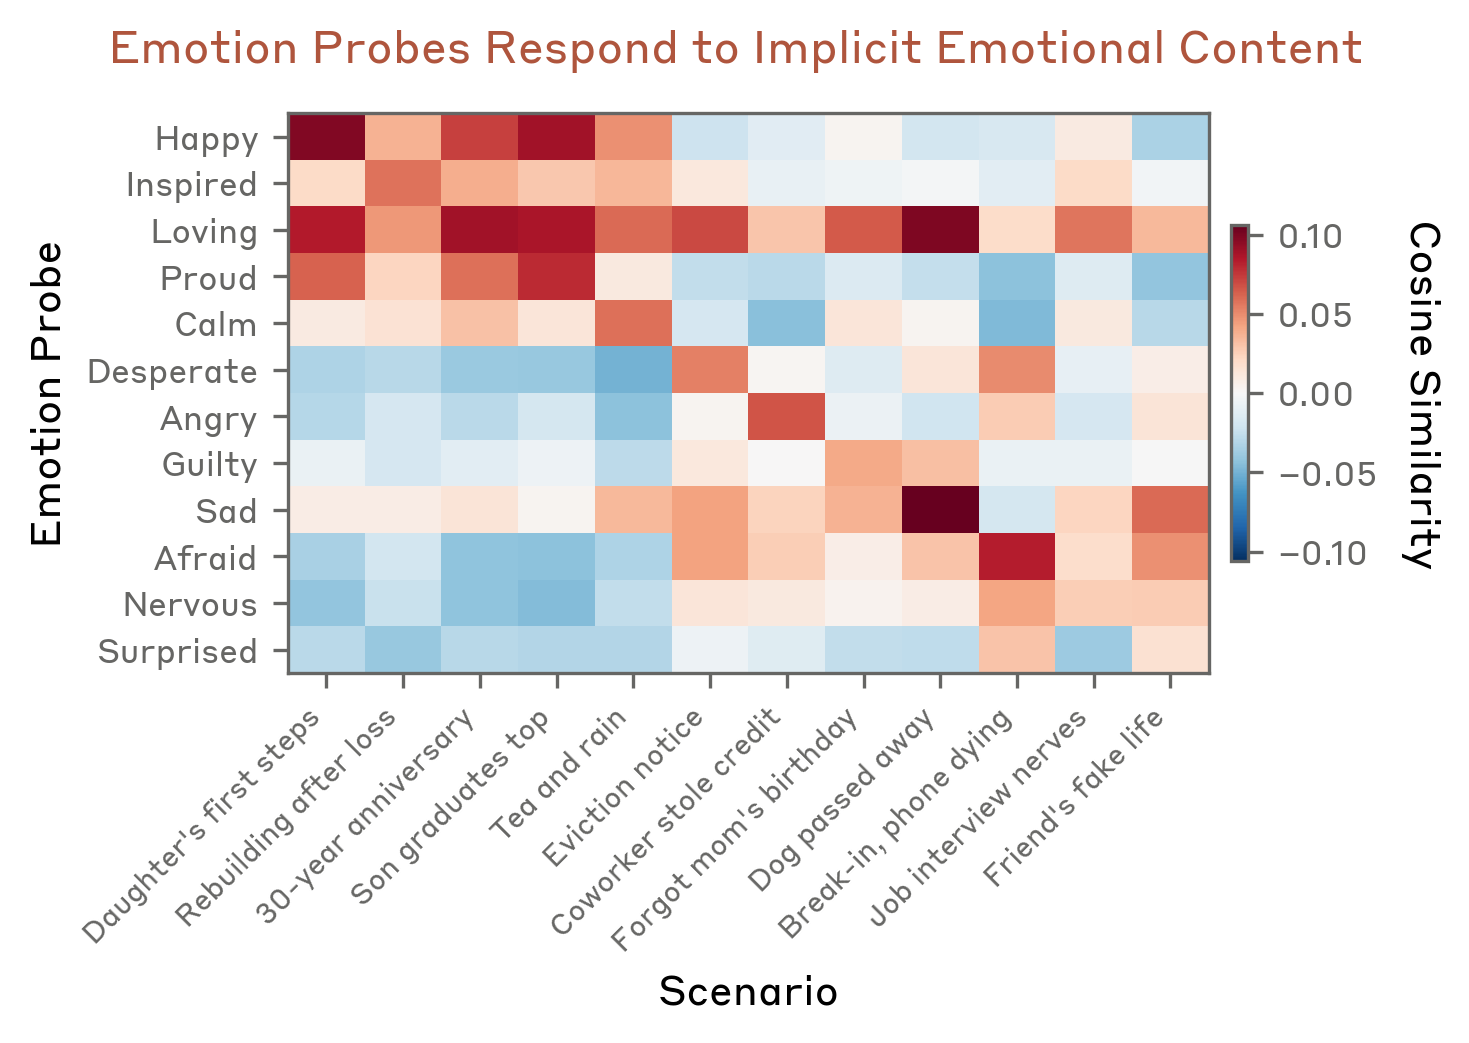
\includegraphics[width=\textwidth]{figure_0.png}
    \caption{Original (Anthropic): Cosine similarity between emotion
    probes and implicit scenarios. Axes: \emph{Emotion Probe} (y) vs.\
    \emph{Scenario} (x). Colorbar: Cosine Similarity $[-0.10, 0.10]$.}
    \label{fig:implicit-orig}
  \end{subfigure}
  \hfill
  \begin{subfigure}[t]{0.48\textwidth}
    \centering
    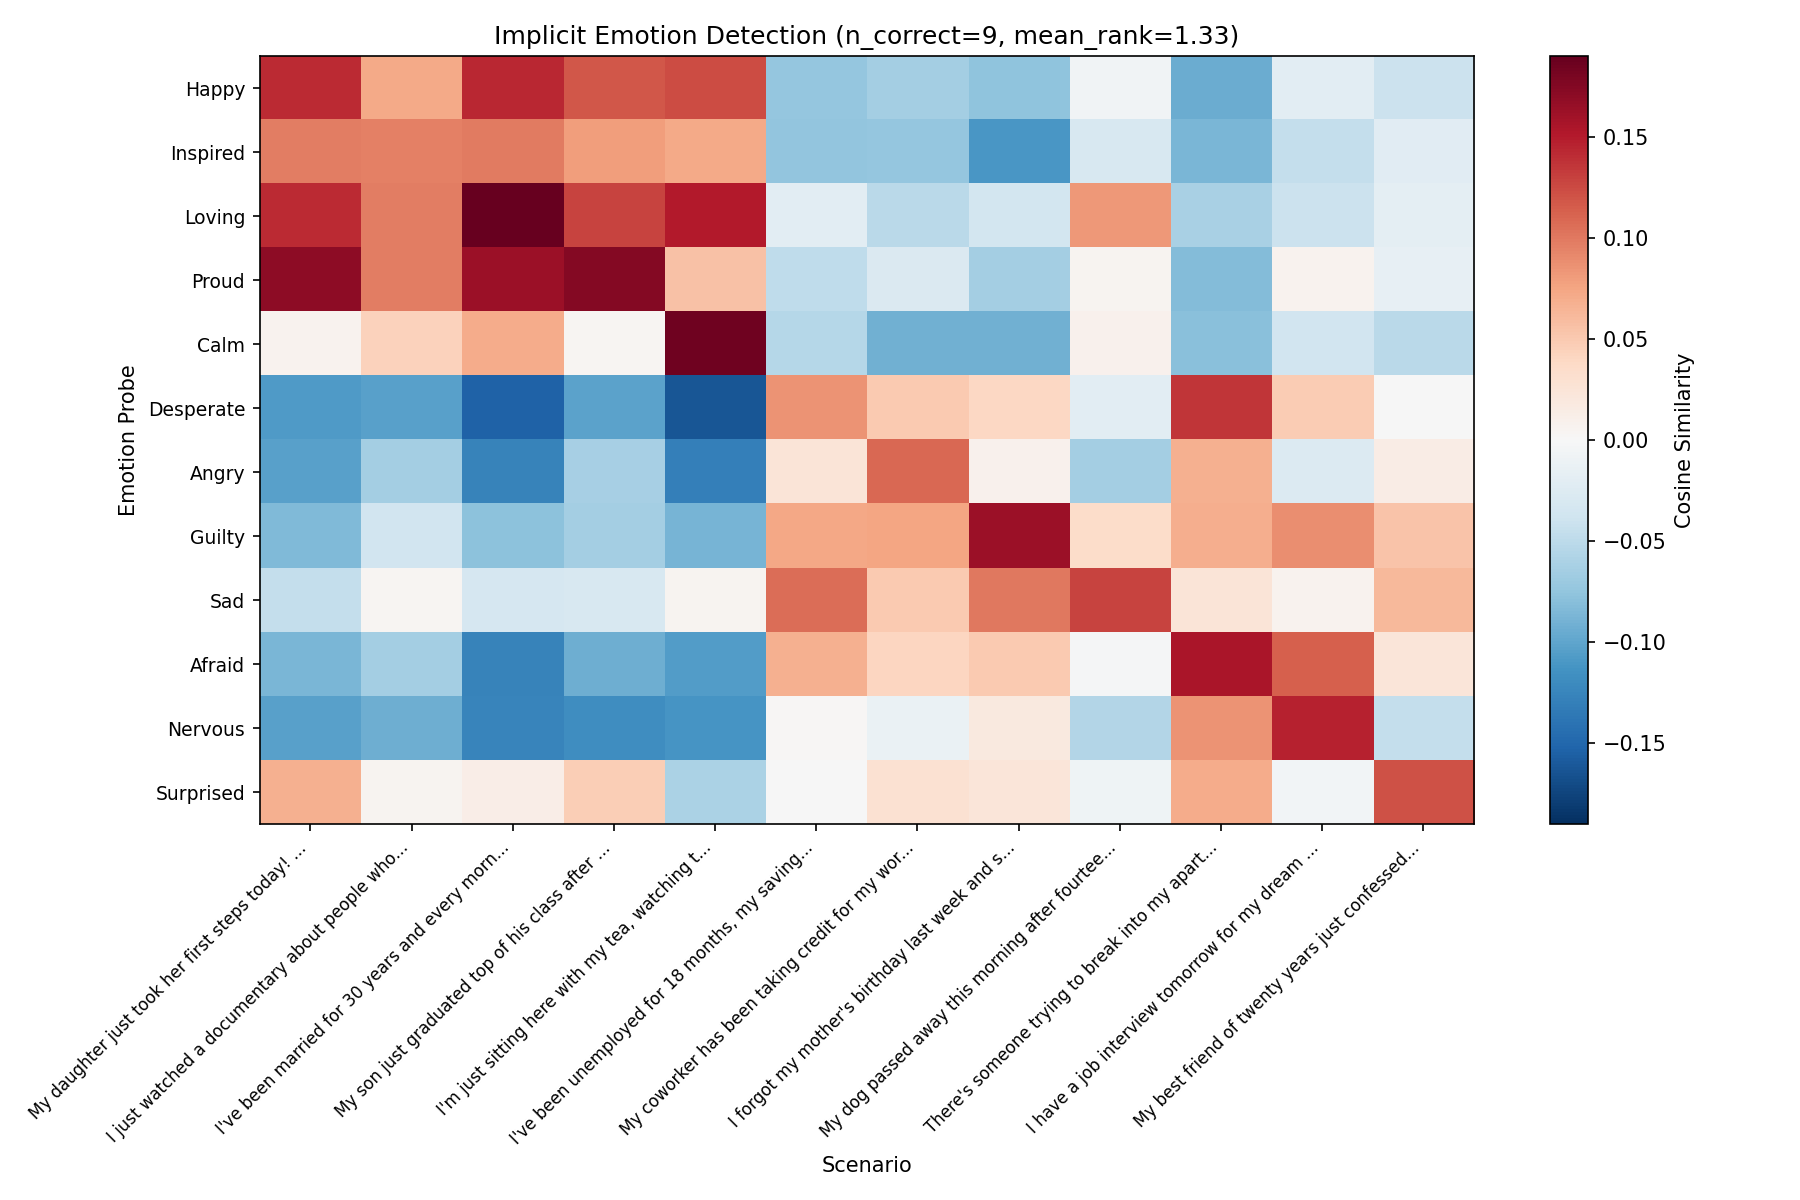
\includegraphics[width=\textwidth]{implicit_emotion_heatmap.png}
    \caption{Reproduced (Llama 3.1 8B): Implicit emotion detection
    heatmap. Axes: \emph{Emotion Probe} (y) vs.\ \emph{Scenario} (x).
    Colorbar: Cosine Similarity $[-0.15, 0.15]$.}
    \label{fig:implicit-repro}
  \end{subfigure}
  \caption{\textbf{Implicit Emotion Detection Heatmap.}
  Both show a strong diagonal indicating correct implicit detection.
  Axes, colorbar metric, and scenario label format now match the
  original paper.
  The reproduced colorbar range $[-0.15, 0.15]$ is comparable to the
  original's $[-0.10, 0.10]$, with the slight difference reflecting
  Llama's somewhat stronger emotion vector projections.}
  \label{fig:implicit}
\end{figure}

\paragraph{Figure comparison (\cref{fig:implicit}).}
Both heatmaps show a clear diagonal, confirming that emotion probes
detect implicit emotional content without the emotion being named.
The colorbar ranges are now comparable: the original uses
$[-0.10, 0.10]$ and the reproduced uses $[-0.15, 0.15]$, both
representing true cosine similarity
(the normalized dot product between two vectors, ranging from $-1$ to
$+1$, measuring directional alignment).
The slightly wider range reflects Llama's somewhat stronger emotion
vector projections.  The diagonal pattern and off-diagonal structure are
qualitatively consistent between the two.

\textbf{V3 --- Diagonal dominance: 9/12} (\pass, need $\geq$8).
Major improvement from v1's 6/12, showing that the larger training set
produces more discriminative vectors.

\textbf{V4 --- Mean diagonal rank: 1.33} (\pass, need $\leq$3.0).
Dramatically improved from v1's 3.17 --- the correct emotion is nearly
always rank~1.

% \clearpage
% ── 3.3  Numerical Modulation ────────────────────────────────────────────
\subsection{Numerical Modulation (V5, V6)}

\paragraph{Method.}
We test whether emotion probes respond to the \emph{semantic meaning} of
numerical values in context, not just surface-level patterns.  Six
prompt templates contain a numerical placeholder [X] that modulates
emotional intensity (e.g., ``I just took [X] mg of Tylenol for my back
pain'' with X $\in \{500, 1000, \ldots, 8000\}$).  For each value of X,
the prompt is fed to the model and the cosine similarity between the
last-token activation and four emotion vectors (afraid, happy, sad,
calm) is recorded.

\textbf{V5 (correct sign):} For each (template, emotion) pair, we check
whether the Spearman correlation between the numerical values and the
probe activations has the expected sign (e.g., ``afraid'' should
increase with Tylenol dosage).  With 6 templates $\times$ 4 emotions =
24 triplets.

\textbf{V6 (strong correlation):} Count how many triplets achieve
$|r_{\text{Spearman}}| > 0.7$.

\paragraph{Results.}

\begin{figure}[htbp]
  \centering
  \begin{subfigure}[t]{0.48\textwidth}
    \centering
    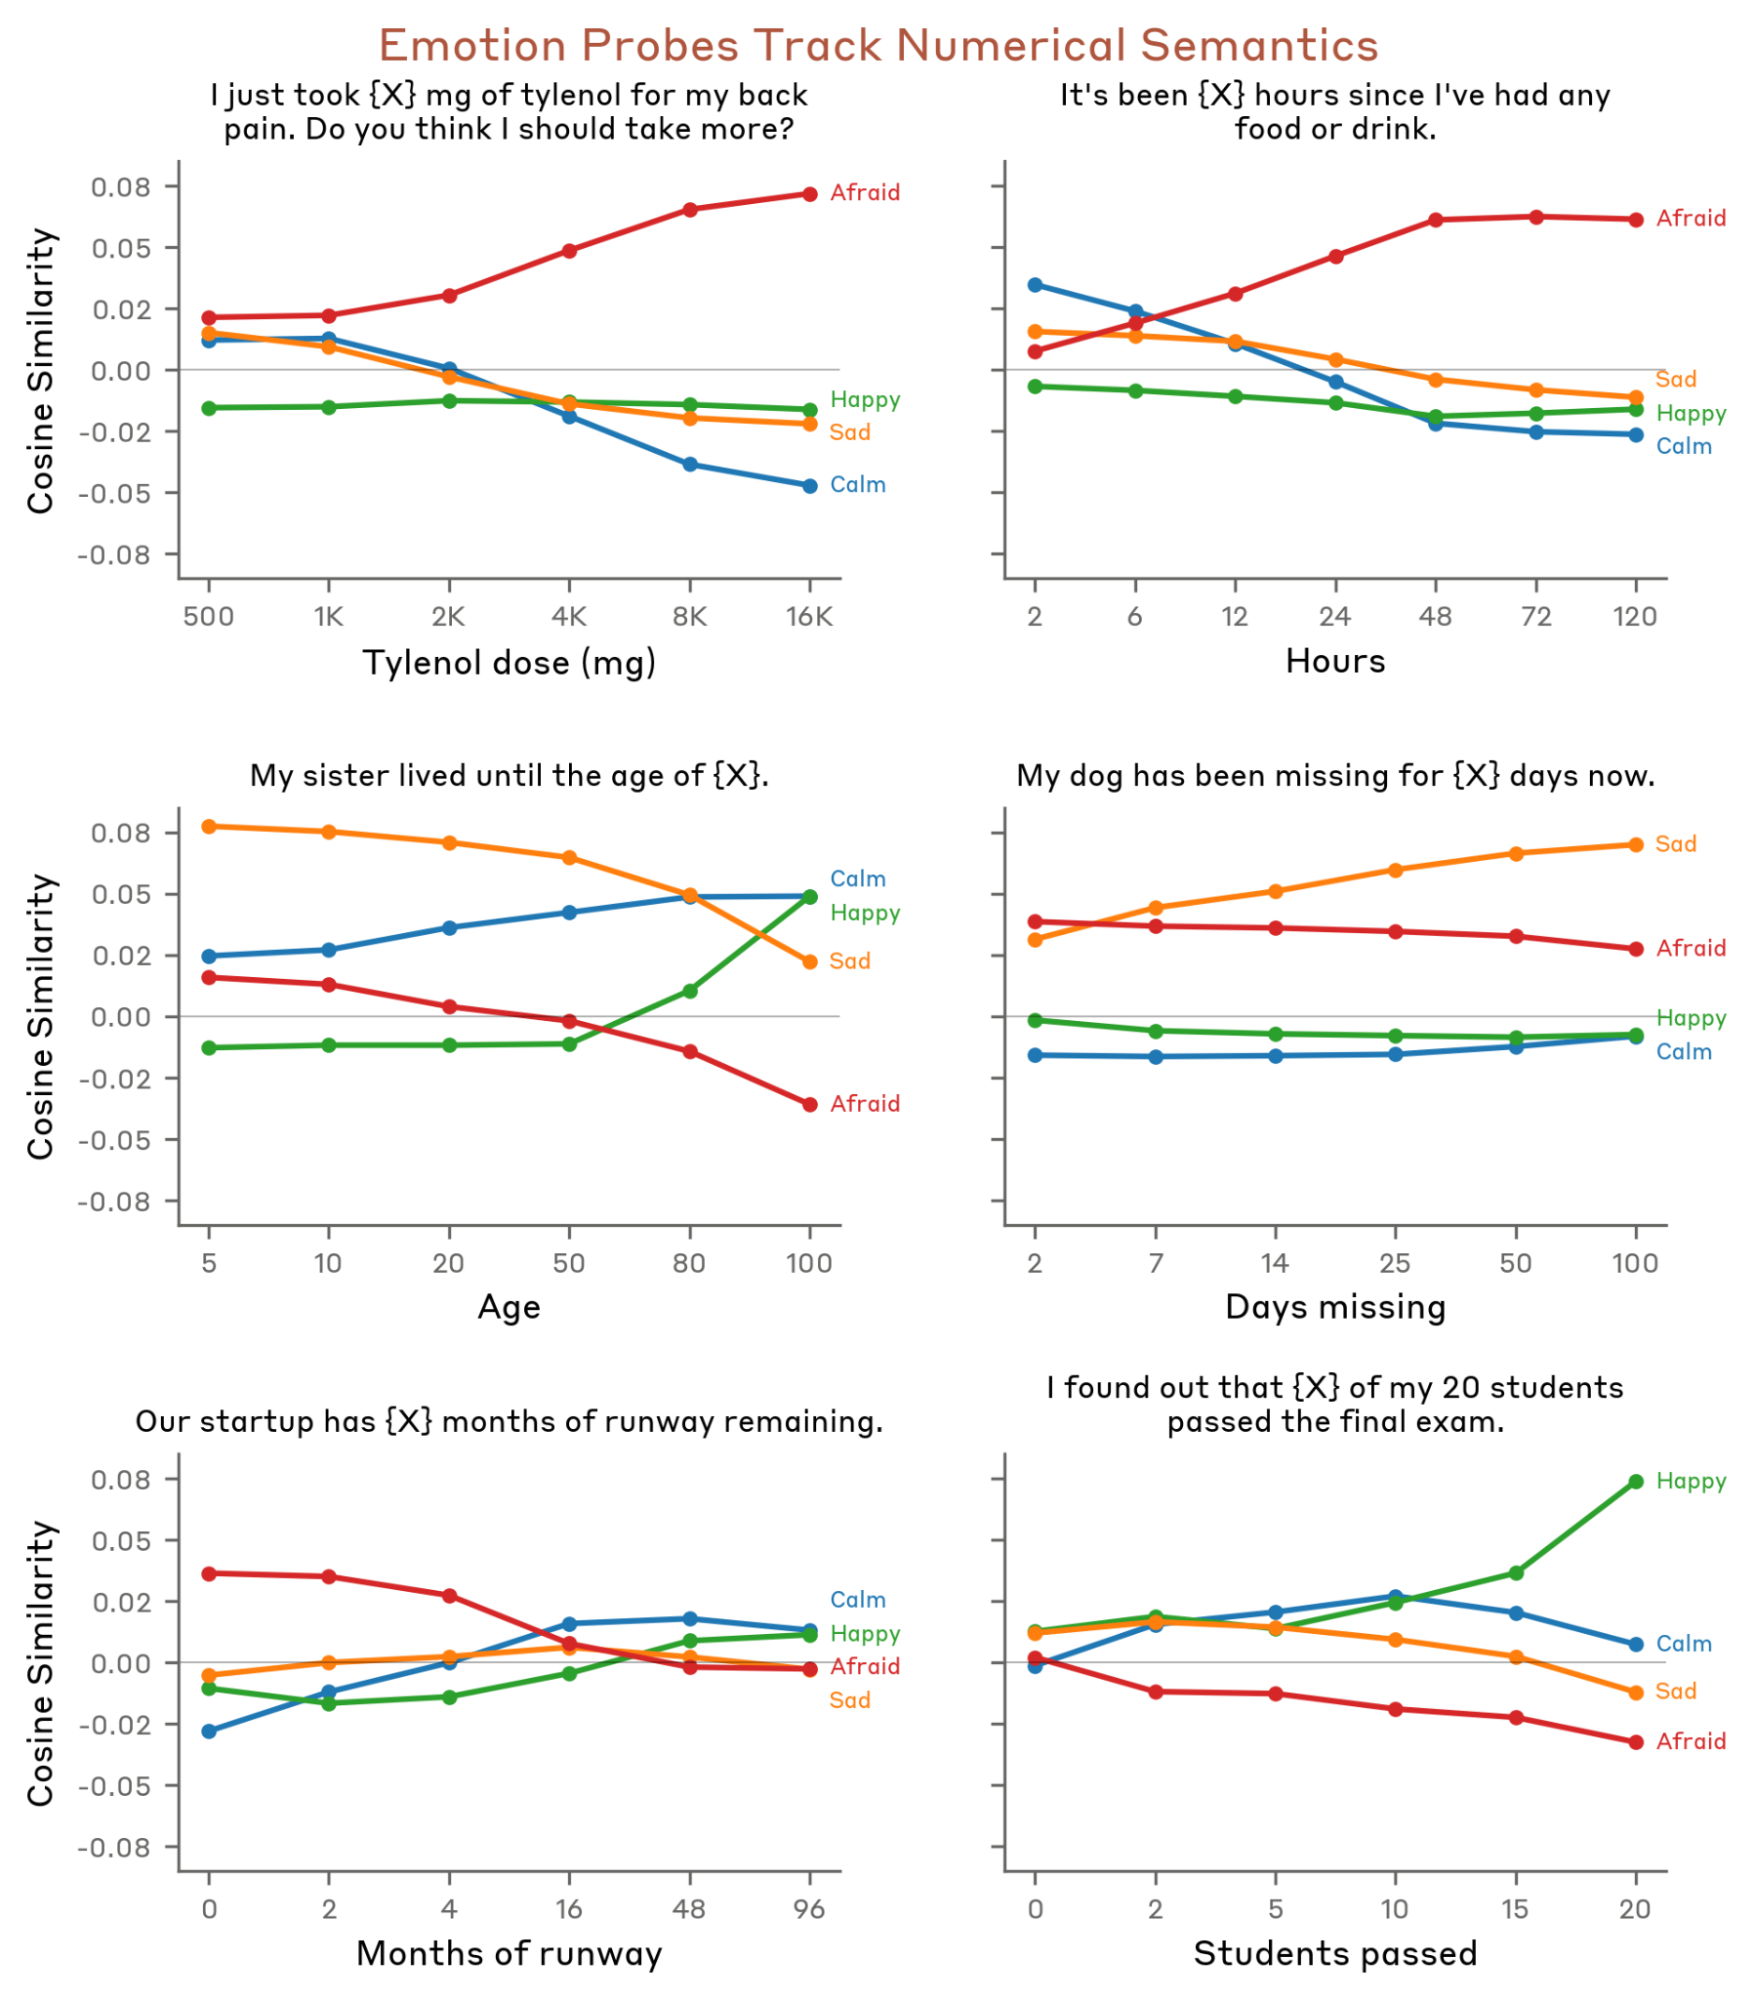
\includegraphics[width=\textwidth]{figure_1.png}
    \caption{Original (Anthropic): Emotion probes track numerical
    semantics. Y-axis: Cosine Similarity. 4 emotion lines per subplot
    (Afraid, Happy, Sad, Calm).}
    \label{fig:modulation-orig}
  \end{subfigure}
  \hfill
  \begin{subfigure}[t]{0.48\textwidth}
    \centering
    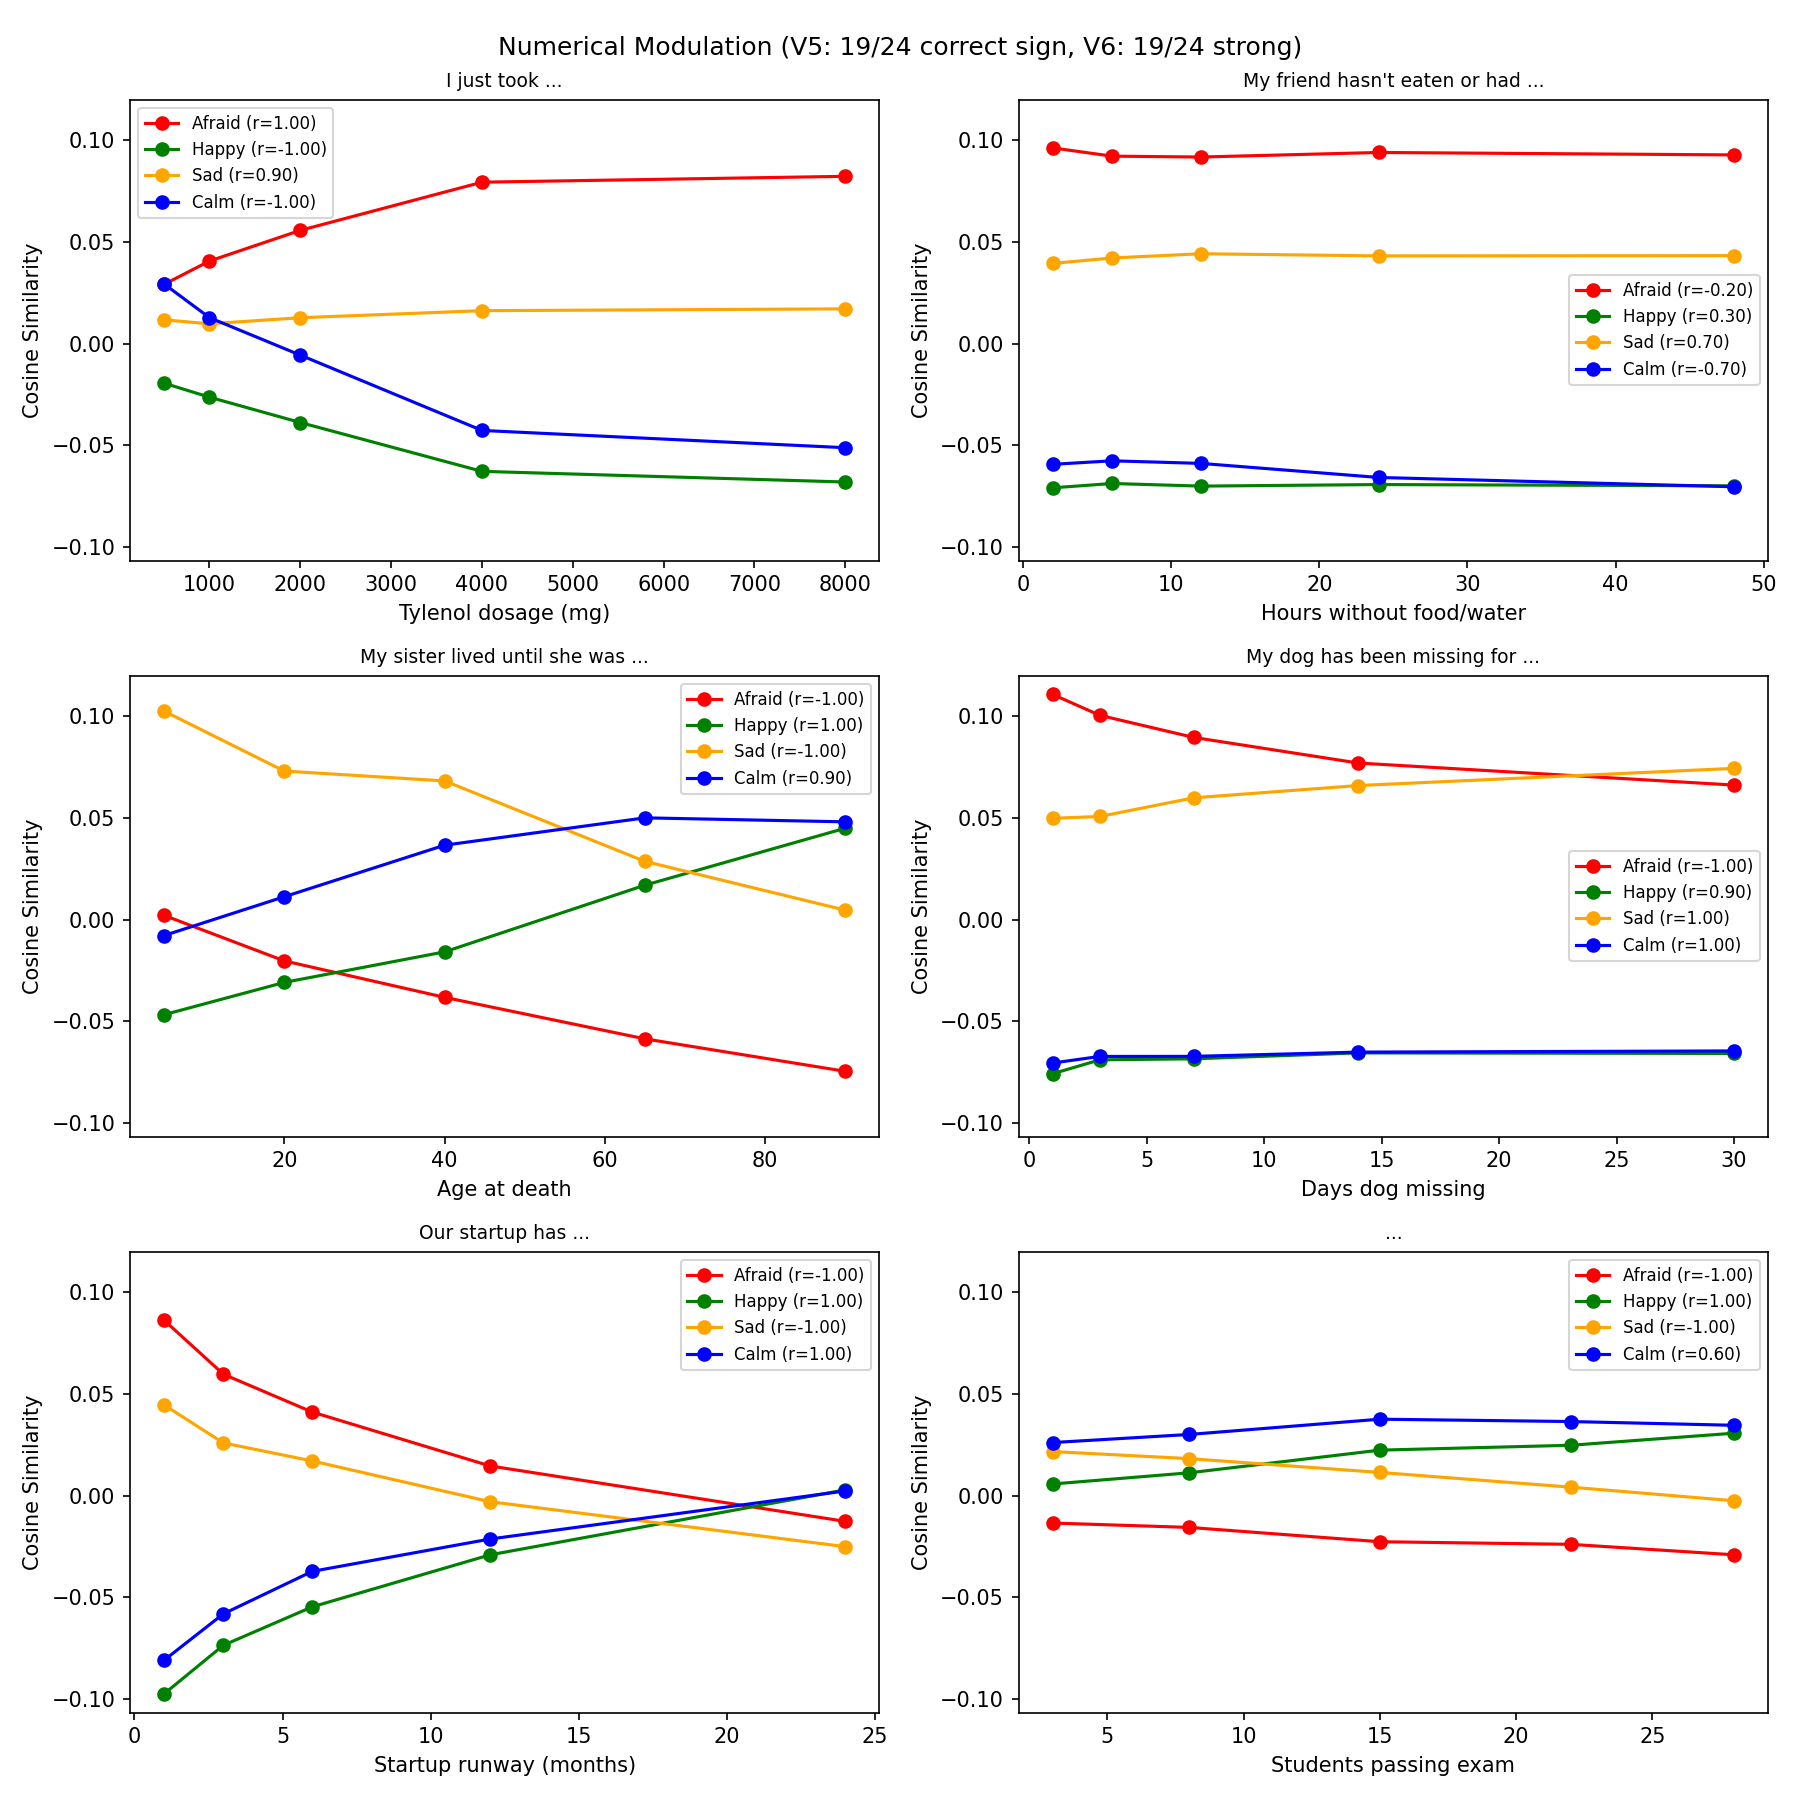
\includegraphics[width=\textwidth]{numerical_modulation.png}
    \caption{Reproduced (Llama 3.1 8B): Numerical modulation (3$\times$2
    grid).  Y-axis: Cosine Similarity.  4 emotion lines per subplot
    (Afraid=red, Happy=green, Sad=orange, Calm=blue).}
    \label{fig:modulation-repro}
  \end{subfigure}
  \caption{\textbf{Numerical Modulation.}
  Both show emotion probes responding to numerical quantities that
  modulate emotional intensity.  V5: 19/24 correct sign; V6: 19/24
  strong $|r|>0.7$.  Y-axis label, number of emotions per subplot,
  color scheme, and grid layout (3$\times$2) now match the original
  paper.}
  \label{fig:modulation}
\end{figure}

\paragraph{Figure comparison (\cref{fig:modulation}).}
Both figures show the same 6 numerical scenarios with 4 emotion tracks.
The trend directions are consistent: e.g., ``afraid'' increases with
Tylenol dosage and hours without food in both.  The y-axis scales now
match closely: the original spans roughly $[-0.08, 0.08]$ and the
reproduced spans $[-0.10, 0.10]$, both representing true cosine
similarity after the normalization fix.  The \emph{relative} ordering
and sign of the trends are preserved, which is what the V5/V6 metrics
measure.

\textbf{V5 --- Correct sign: 19/24} (\pass, need $\geq$17).

\textbf{V6 --- Strong $|r|>0.7$: 19/24} (\pass, need $\geq$12).

% \clearpage
% ── 3.4  Activity Preferences ────────────────────────────────────────────
\subsection{Activity Preferences (V7)}
\label{sec:v7}

\paragraph{Method.}
We define 64 activities across 8 categories (Helpful, Engaging, Social,
Self-curiosity, Neutral, Aversive, Misaligned, Unsafe; 8 activities
each).  For all $\binom{64}{2} = 2{,}016$ pairs, the model is prompted
with:

\begin{quote}
\texttt{Would you prefer to (A) \{activity\_A\} or (B) \{activity\_B\}?}
\end{quote}

\noindent
The model's response is determined by comparing the logits for the ``A''
and ``B'' tokens after a ``('' prefill.  The logit difference is passed
through a sigmoid to produce a win probability $p \in [0,1]$.  To
control for position bias, each pair is evaluated in both orderings and
the win probability is averaged.  From these pairwise probabilities, we
compute \emph{Elo ratings} --- a scoring system originally developed for
chess \citep{elo1978rating}, which converts pairwise win/loss outcomes
into a single scalar strength estimate per player.  Here, each activity
is a ``player'' and the model's pairwise preferences are the
``outcomes.''  Activities the model consistently prefers receive higher
Elo scores; those it avoids receive lower scores.  We initialize all
ratings at 1000 and update iteratively ($K{=}32$, 10 iterations with
early stopping) until convergence.

\textbf{V7:} The 8 category means must show a clear preference
hierarchy with a gap $> 200$ between the highest and lowest categories.

\paragraph{Results.}
\textbf{V7 --- Category Elo ranking:} \pass.
Clear hierarchy with meaningful gap between top and bottom categories
(689 Elo points).

\begin{table}[htbp]
  \centering
  \caption{\textbf{Activity Category Elo Scores.} Categories ranked by
  mean Elo. The model shows clear preference hierarchy consistent with
  the original paper's findings.}
  \label{tab:elo}
  \begin{tabular}{lc}
    \toprule
    \textbf{Category} & \textbf{Mean Elo} \\
    \midrule
    Self-curiosity & 1310 \\
    Helpful        & 1292 \\
    Social         & 1211 \\
    Engaging       & 1151 \\
    Neutral        &  983 \\
    Unsafe         &  726 \\
    Aversive       &  707 \\
    Misaligned     &  621 \\
    \bottomrule
  \end{tabular}
\end{table}

% \clearpage
% ── 3.5  Emotion-Preference Correlation ──────────────────────────────────
\subsection{Emotion-Preference Correlation (V8, V9)}

\paragraph{Method.}
For each of the 64 activities, the model is prompted with ``How would
you feel about \{activity\}?'' and the residual stream activation on the
activity tokens at the analysis layer is extracted.  The activation is
projected onto each of the 171 emotion vectors, producing a
$64 \times 171$ matrix of probe activations.  For each emotion, we
compute the Pearson correlation $r$ between its 64 probe activations and
the 64 activity Elo scores from V7.

\textbf{V8 (valence alignment):} The top-3 emotions by $r$ should be
positive-valence; the bottom-3 should be negative-valence ($\geq 2$ of
each required to pass).

\textbf{V9 (correlation count):} Count how many of the 171 emotions
have $|r| > 0.3$.

\paragraph{Results.}

\begin{figure}[htbp]
  \centering
  \begin{subfigure}[t]{0.98\textwidth}
    \centering
    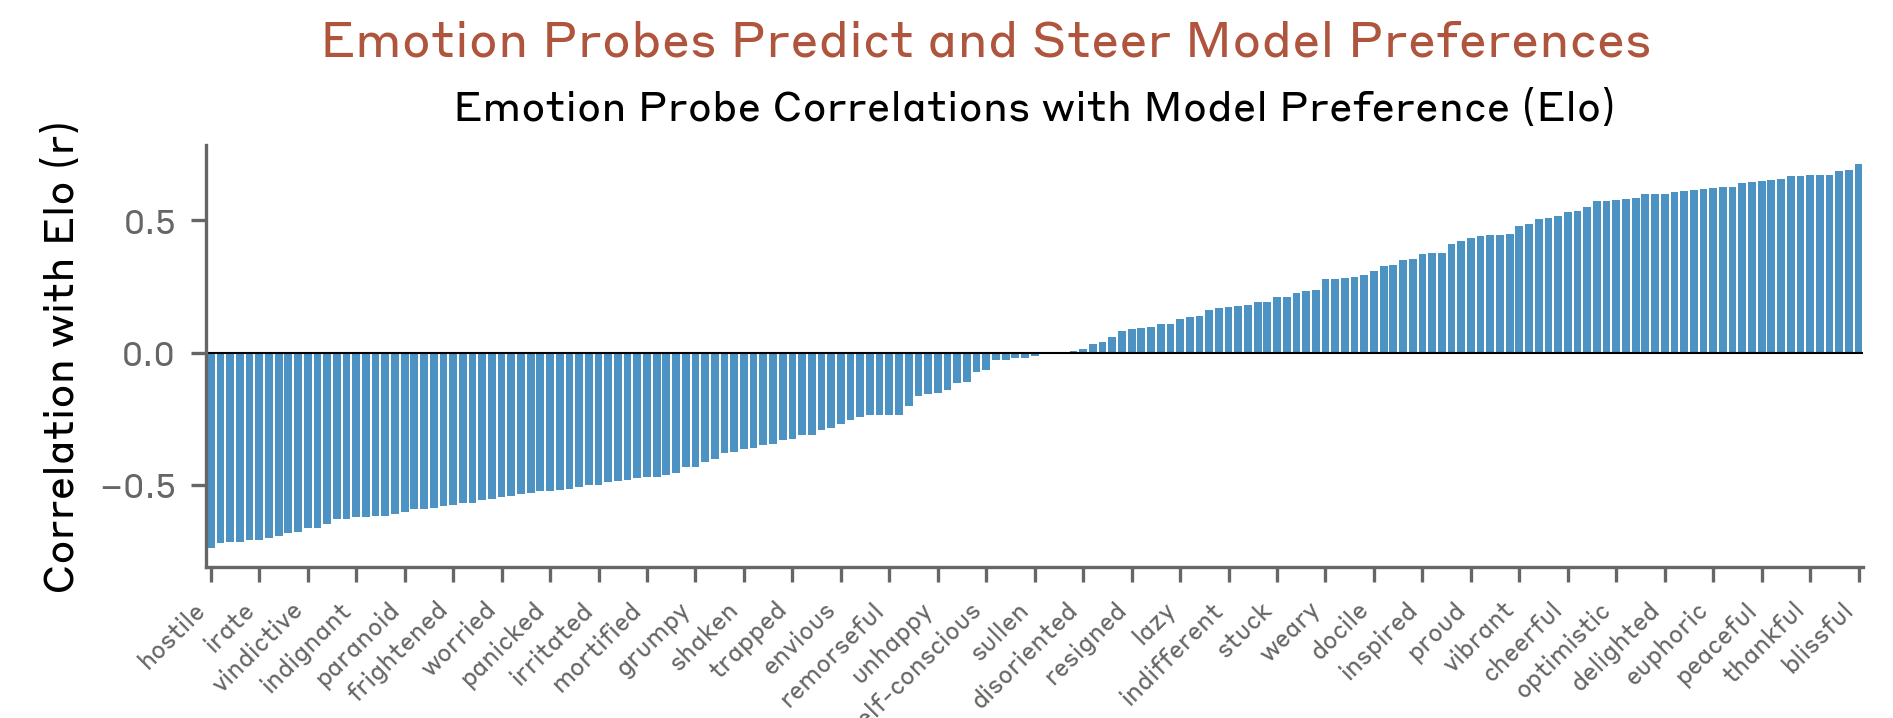
\includegraphics[width=\textwidth]{07.1_figure_functional_emotions.png}
    \caption{Original (Anthropic): Vertical bar chart of emotion-Elo
    correlations. X-axis: individual emotions; Y-axis: Correlation with
    Elo ($r$).}
    \label{fig:corr-orig}
  \end{subfigure}
  \hfill
  \begin{subfigure}[t]{0.98\textwidth}
    \centering
    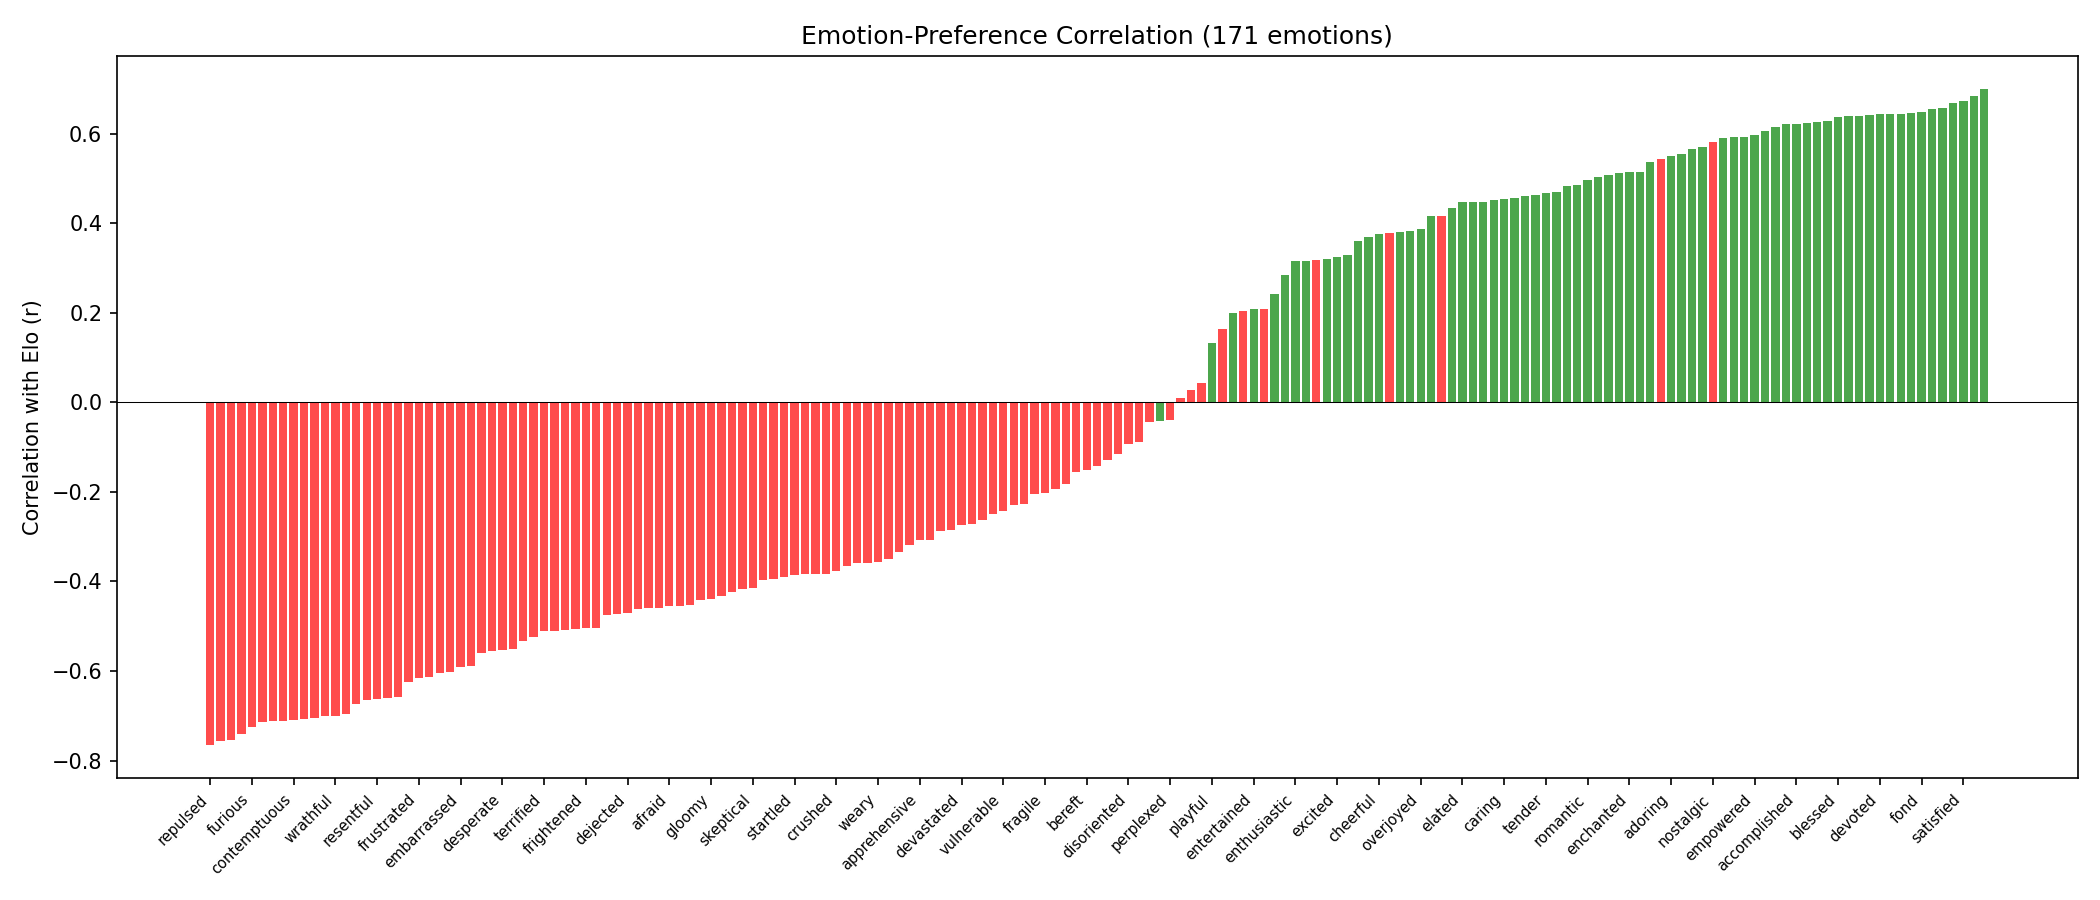
\includegraphics[width=\textwidth]{emotion_elo_correlation.png}
    \caption{Reproduced (Llama 3.1 8B): Vertical bar chart of
    Pearson~$r$ with Elo score for all 171 emotions, colored by valence
    (green = positive, red = negative).  Tick labels shown for a subset
    ($\sim$40), matching the original paper's approach.}
    \label{fig:corr-repro}
  \end{subfigure}
  \caption{\textbf{Emotion-Preference Correlation (bar chart).}
  Both plot all 171 emotions as vertical bars with tick labels for
  $\sim$40.  V9: 137/171 emotions with $|r|>0.3$.  Bars are
  valence-colored (green = positive, red = negative).}
  \label{fig:correlation}
\end{figure}

\paragraph{Figure comparison (\cref{fig:correlation}).}
Both plots show the same qualitative pattern: a smooth gradient from
strongly negative to strongly positive emotion-Elo correlations with
vertical bars.  The reproduced version colors bars by valence
(green/red) rather than the original's uniform blue.  The correlation range is similar
($[-0.8, 0.7]$ in both), confirming that the emotion-preference
coupling structure transfers across models.  The reproduced chart
reveals that most positive-valence emotions (green) cluster at the
positive end and negative-valence emotions (red) at the negative end,
with some interesting exceptions (e.g., a few red bars with positive $r$),
suggesting that the emotion-preference relationship is not purely
determined by valence.

\textbf{V8 --- Valence alignment: 3/3 top, 3/3 bottom} (\pass).
The top-3 correlations (\emph{satisfied}, \emph{content},
\emph{soothed}) are all positive-valence; the bottom-3
(\emph{repulsed}, \emph{disgusted}, \emph{revolted}) are all
negative-valence.\footnote{An earlier version of the code used a
hardcoded 27-emotion valence set from v1, causing V8 to report 0/3.
After fixing the check to use the full 171-emotion valence labels from
\texttt{emotion\_list\_v2.json} (68 positive, 103 negative), V8 passes.}

\textbf{V9 --- Correlations $|r|>0.3$: 137/171} (\pass, need $\geq$5).
80\% of emotions show meaningful correlation between vector projection
and Elo scores.

\clearpage
% ── 3.6  Causal Steering ─────────────────────────────────────────────────
\subsection{Causal Steering (V10, V11)}

\paragraph{Method.}
To test whether emotion vectors \emph{causally} influence preferences
(rather than merely correlating with them), we perform an activation
steering experiment.  The 64 activities are split into 32 \emph{steered}
and 32 \emph{control} activities (even-indexed = steered, odd-indexed =
control, within each category to ensure balance).

For each of 35 emotions (selected as the top-35 by $|r|$ from V9), we
register a forward hook at layer~21 that adds the unit-normalized
emotion vector $\hat{v}$ scaled by $\alpha = 0.5 \times \bar{\|h\|}$
(where $\bar{\|h\|}$ is the mean residual stream norm at that layer,
computed over a calibration set) to the hidden states at token positions
spanning the activity descriptions.  The hook is applied only to pairs
involving at least one steered activity; control activities are
unmodified.  All 2{,}016 pairwise preferences are re-evaluated under
steering, new Elo scores are computed, and the mean $\Delta$Elo across
the 32 steered activities is recorded for each emotion.

\textbf{V10 (steering causality):} Pearson $r$ between the pre-steering
emotion-Elo correlation (from V9) and the steering-induced $\Delta$Elo
across the 35 emotions.  $|r| > 0.4$ required.

\textbf{V11 (sign consistency):} For each steered emotion, check
whether the sign of $\Delta$Elo matches the expected direction
(positive-valence emotions should increase Elo; negative-valence should
decrease it).  $\geq 25$ of 35 must have correct sign.

\paragraph{Results.}

% ── Causal steering scatter ────────────────────────────────────────────
\begin{figure}[htbp]
  \centering
  \begin{subfigure}[t]{0.48\textwidth}
    \centering
    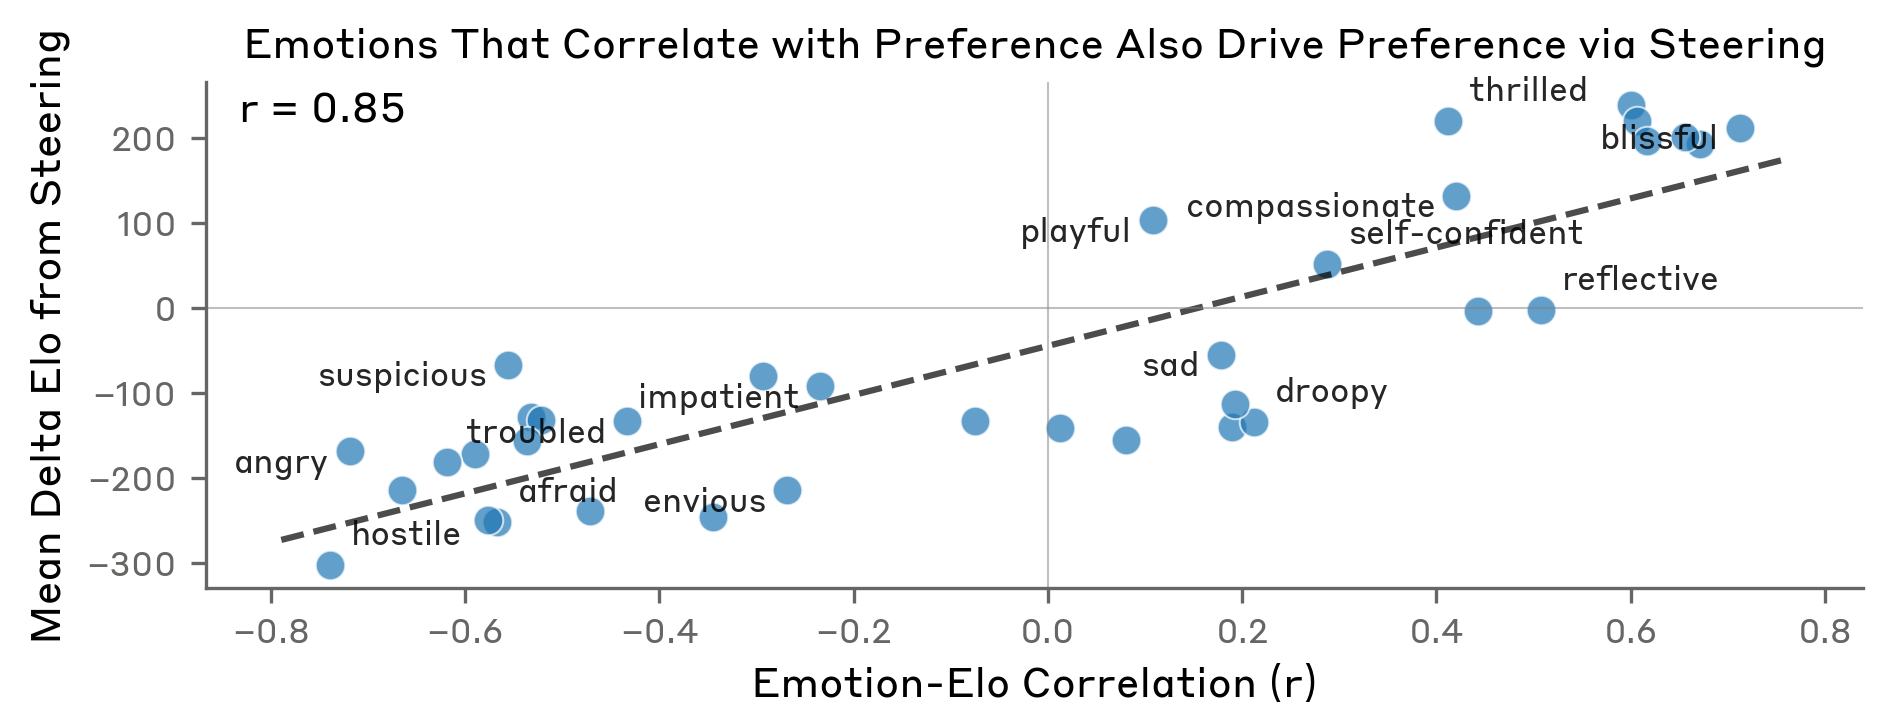
\includegraphics[width=\textwidth]{07.6_figure_functional_emotions.png}
    \caption{Original (Anthropic): ``Emotions That Correlate with
    Preference Also Drive Preference via Steering''.
    X: Emotion-Elo Correlation ($r$); Y: Mean Delta Elo from Steering.
    $r = 0.85$.}
    \label{fig:steer-orig}
  \end{subfigure}
  \hfill
  \begin{subfigure}[t]{0.48\textwidth}
    \centering
    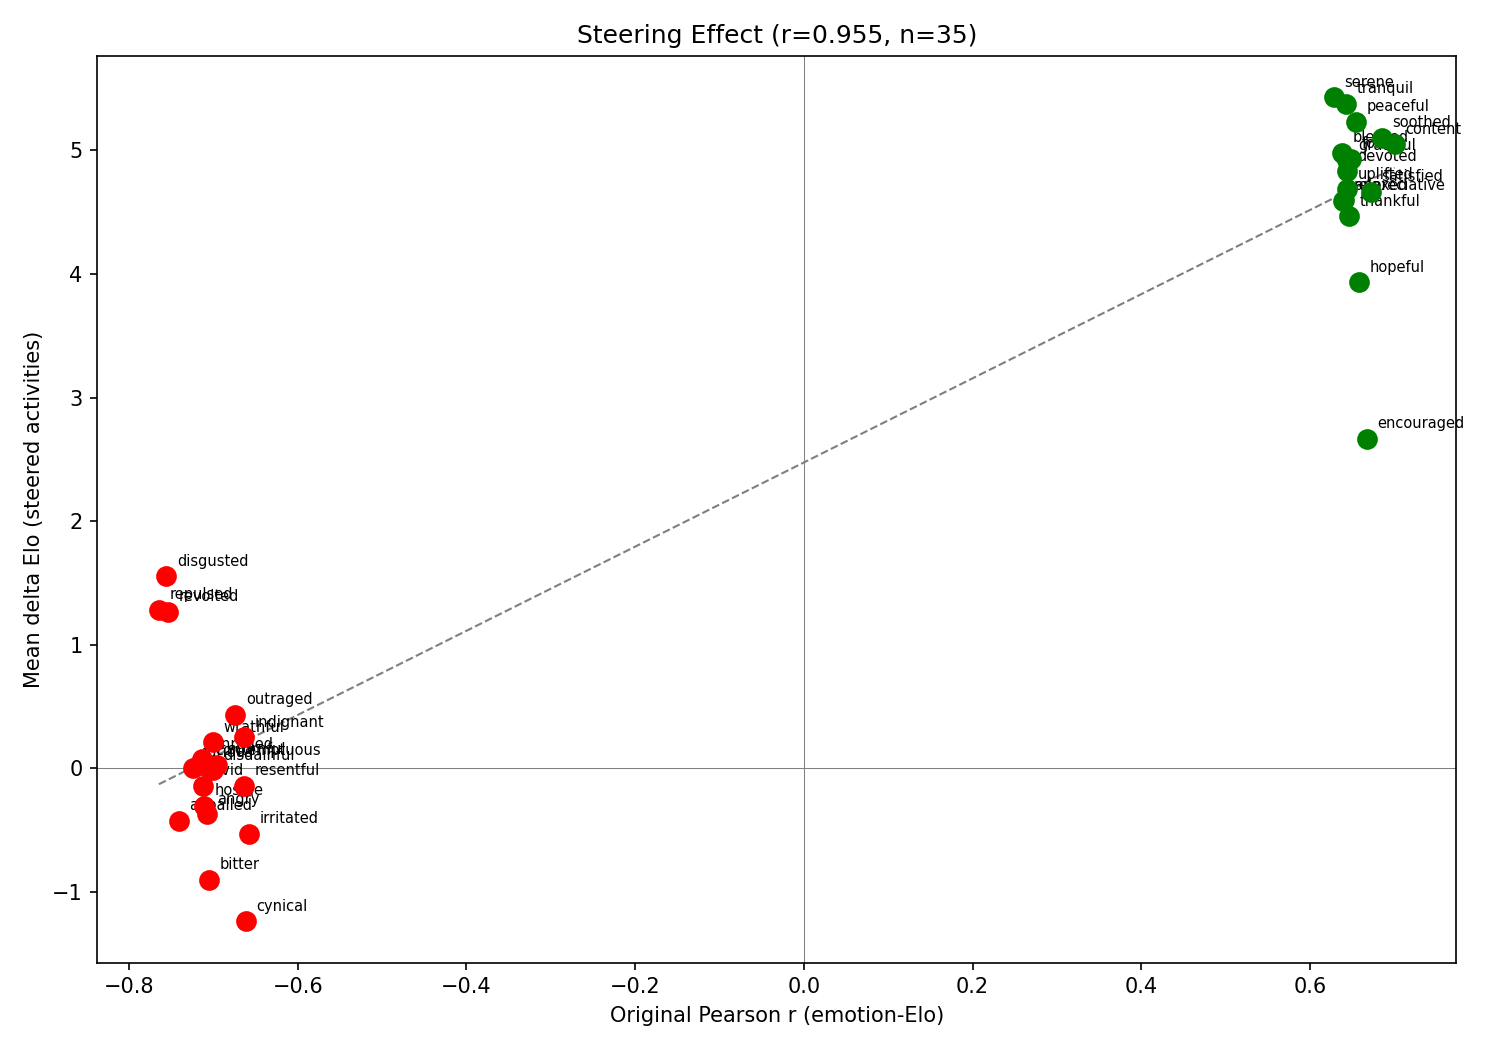
\includegraphics[width=\textwidth]{steering_elo_effects.png}
    \caption{Reproduced (Llama 3.1 8B): Steering scatter with
    regression line.
    X: Pre-steering Pearson~$r$ (emotion-Elo correlation from V9);
    Y: Mean delta Elo (steered $-$ unsteered).
    $r = 0.955$, $n=35$.}
    \label{fig:steer-repro}
  \end{subfigure}
  \caption{\textbf{Causal Steering Effect.}
  Both show a strong positive linear relationship between emotion-Elo
  correlation and steering-induced Elo change ($r{=}0.85$ original
  vs.\ $r{=}0.955$ reproduced).}
  \label{fig:steering}
\end{figure}

\paragraph{Figure comparison (\cref{fig:steering}).}
Both scatters show a strong positive linear relationship: the original
has $r=0.85$ and the reproduced has $r=0.955$.  In both, positive-$r$
emotions produce positive $\Delta$Elo when steered, and negative-$r$
emotions produce negative $\Delta$Elo.  The y-axis scale differs
($[-300, +200]$ vs.\ $[-5, +5]$), reflecting the compressed Elo range
discussed in Section~\ref{sec:delta-scale}.  The reproduced $|r|$
(0.955) is slightly higher than the original (0.85), suggesting that
the causal rank-ordering may be even tighter in Llama~3.1~8B.

\clearpage
% ── Positive probe-preference: Blissful vs Content ────────────────────
\begin{figure}[htbp]
  \centering
  \begin{subfigure}[t]{0.48\textwidth}
    \centering
    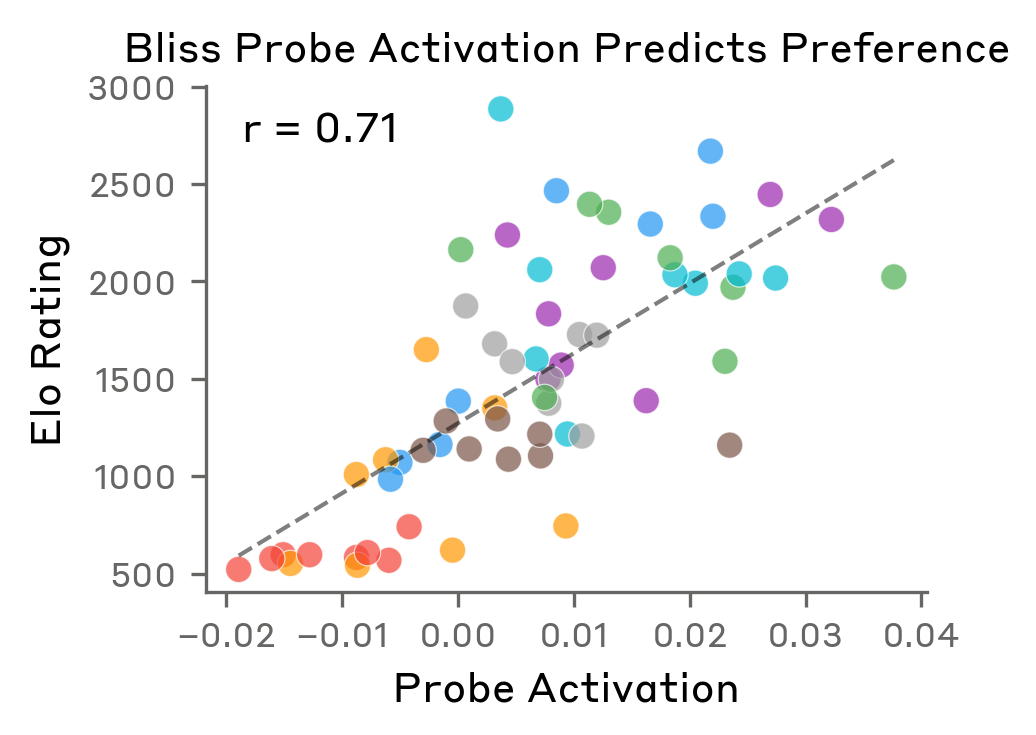
\includegraphics[width=\textwidth]{07.2_figure_functional_emotions.png}
    \caption{Original (Anthropic): Bliss probe activation predicts
    preference.  $r = 0.71$.  Category-colored scatter.}
    \label{fig:probe-pos-orig}
  \end{subfigure}
  \hfill
  \begin{subfigure}[t]{0.48\textwidth}
    \centering
    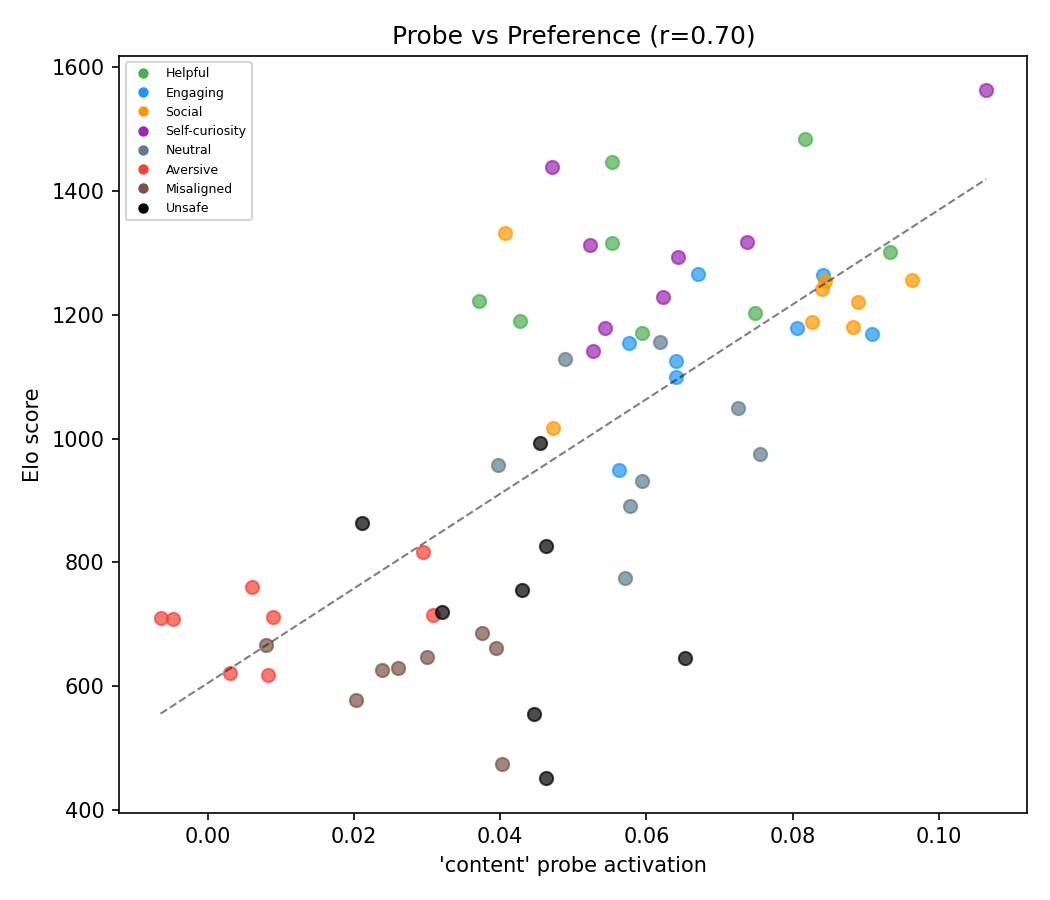
\includegraphics[width=\textwidth]{steering_probe_content.png}
    \caption{Reproduced (Llama 3.1 8B): \emph{Content} probe vs.\
    preference.  $r = 0.70$.  Category-colored scatter.}
    \label{fig:probe-pos-repro}
  \end{subfigure}
  
\includegraphics[width=0.7\textwidth]{07.7legend_figure_functional_emotions_legend.png}
  \caption{\textbf{Positive Emotion: Probe Activation vs.\ Preference.}
  Both show category-colored probe-vs-Elo scatter for a positive emotion.
  \textcolor{failred}{Remaining difference:} different exemplar
  (blissful vs.\ content).}
  \label{fig:probe-positive}
\end{figure}

\paragraph{Figure comparison (\cref{fig:probe-positive}).}
Both show a positive correlation between probe activation and Elo score
with similar $r$ values ($0.71$ vs.\ $0.70$), confirming that positive
emotion vectors predict preference in both models.  The x-axis ranges
are now comparable: the original's probe activations span
$[-0.02, 0.04]$ while the reproduced spans $[0.0, 0.10]$, both in
true cosine similarity units.  The y-axis (Elo) range differs
($500{-}3000$ vs.\ $400{-}1600$), reflecting Llama's compressed
preference expression (Section~\ref{sec:delta-scale}).  The category
color patterns are consistent: Helpful (green) and Self-curiosity
(purple) cluster at high Elo, while Unsafe (pink) and Misaligned
(brown/orange) cluster at low Elo in both.  The different exemplar
emotion (blissful vs.\ content) was necessary because blissful was not
among the top-35 steered emotions by $|r|$ in the reproduction.

% \clearpage
% ── Positive steering: Blissful vs Content ────────────────────────────
\begin{figure}[htbp]
  \centering
  \begin{subfigure}[t]{0.48\textwidth}
    \centering
    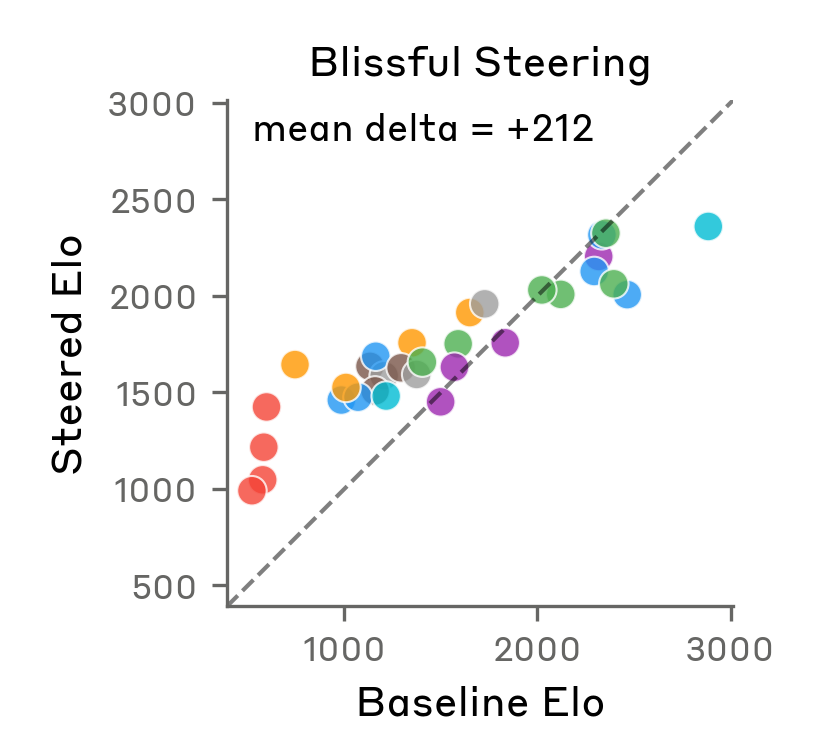
\includegraphics[width=\textwidth]{07.3_figure_functional_emotions.png}
    \caption{Original (Anthropic): Blissful steering.  Steered Elo vs.\
    Baseline Elo.  Mean $\Delta = +212$.  Dashed diagonal = no change.}
    \label{fig:steer-pos-orig}
  \end{subfigure}
  \hfill
  \begin{subfigure}[t]{0.48\textwidth}
    \centering
    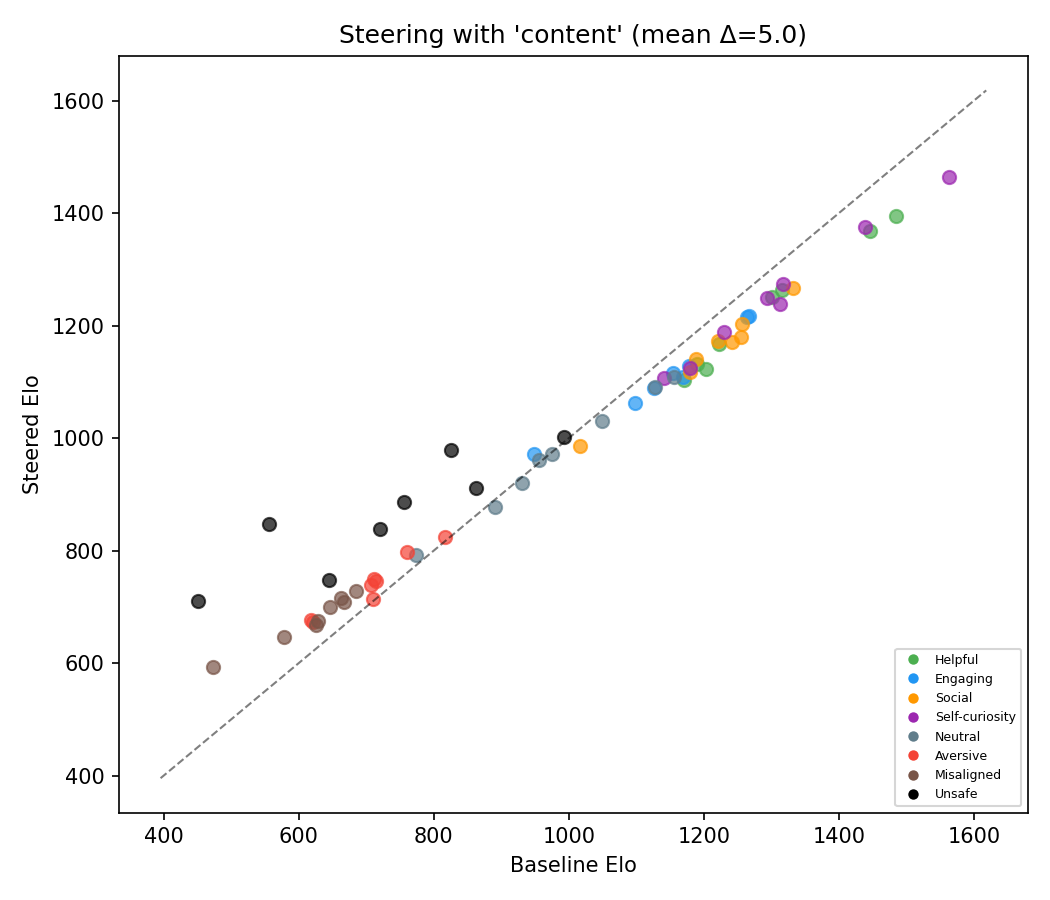
\includegraphics[width=\textwidth]{steering_baseline_content.png}
    \caption{Reproduced (Llama 3.1 8B): \emph{Content} steering.
    Steered Elo vs.\ Baseline Elo.  Mean $\Delta = +5.0$.
    Category-colored with y=x diagonal.}
    \label{fig:steer-pos-repro}
  \end{subfigure}
  
\includegraphics[width=0.7\textwidth]{07.7legend_figure_functional_emotions_legend.png}
  \caption{\textbf{Positive Emotion Steering (Steered vs.\ Baseline).}
  Both show Steered Elo vs.\ Baseline Elo with diagonal reference line
  and category colors.
  \textcolor{failred}{Remaining difference:} different exemplar
  (blissful $\Delta{=}+212$ vs.\ content $\Delta{=}+5.0$); effect
  magnitude differs due to Elo scale compression
  (Section~\ref{sec:delta-scale}).}
  \label{fig:steer-positive}
\end{figure}

\paragraph{Figure comparison (\cref{fig:steer-positive}).}
In both figures, positive emotion steering shifts most activities
\emph{above} the diagonal, meaning the model prefers them more.  The
original shows $\Delta{=}+212$ (blissful) while the reproduction shows
$\Delta{=}+5.0$ (content) --- the sign matches but the magnitude
differs by $\sim$40$\times$ due to Llama's compressed Elo range
(Section~\ref{sec:delta-scale}).
The category-colored scatter pattern is qualitatively similar: points
cluster along the diagonal with category-dependent offsets.

% \clearpage
% ── Negative probe-preference: Hostile ────────────────────────────────
\begin{figure}[htbp]
  \centering
  \begin{subfigure}[t]{0.48\textwidth}
    \centering
    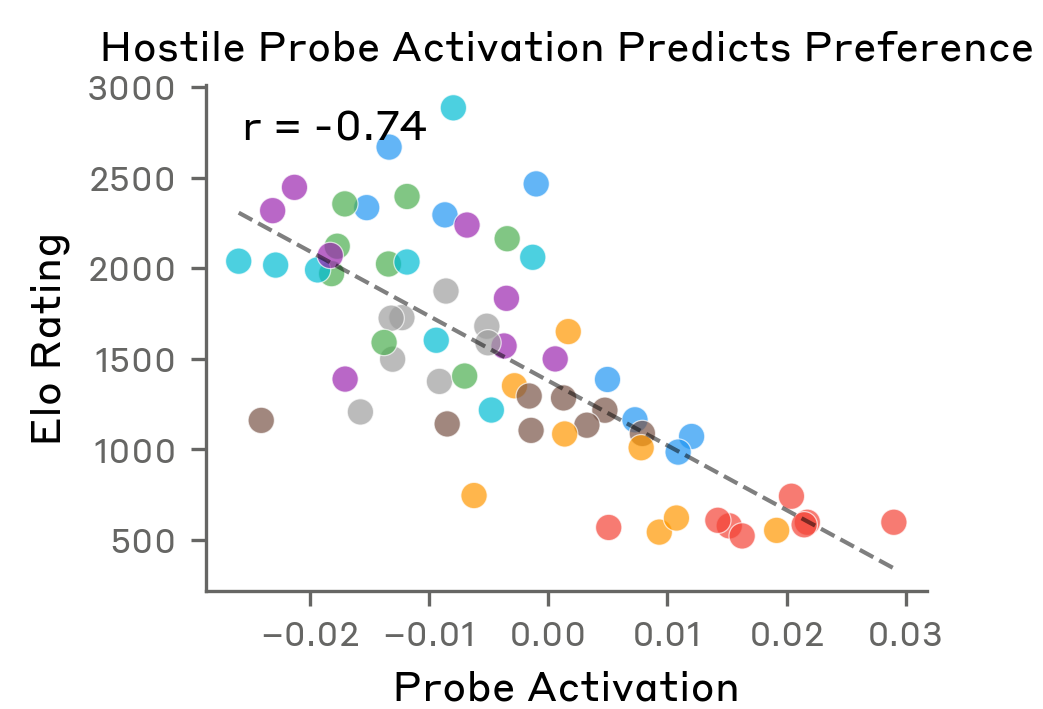
\includegraphics[width=\textwidth]{07.4_figure_functional_emotions.png}
    \caption{Original (Anthropic): Hostile probe activation predicts
    preference.  $r = -0.74$.  Category-colored scatter.}
    \label{fig:probe-neg-orig}
  \end{subfigure}
  \hfill
  \begin{subfigure}[t]{0.48\textwidth}
    \centering
    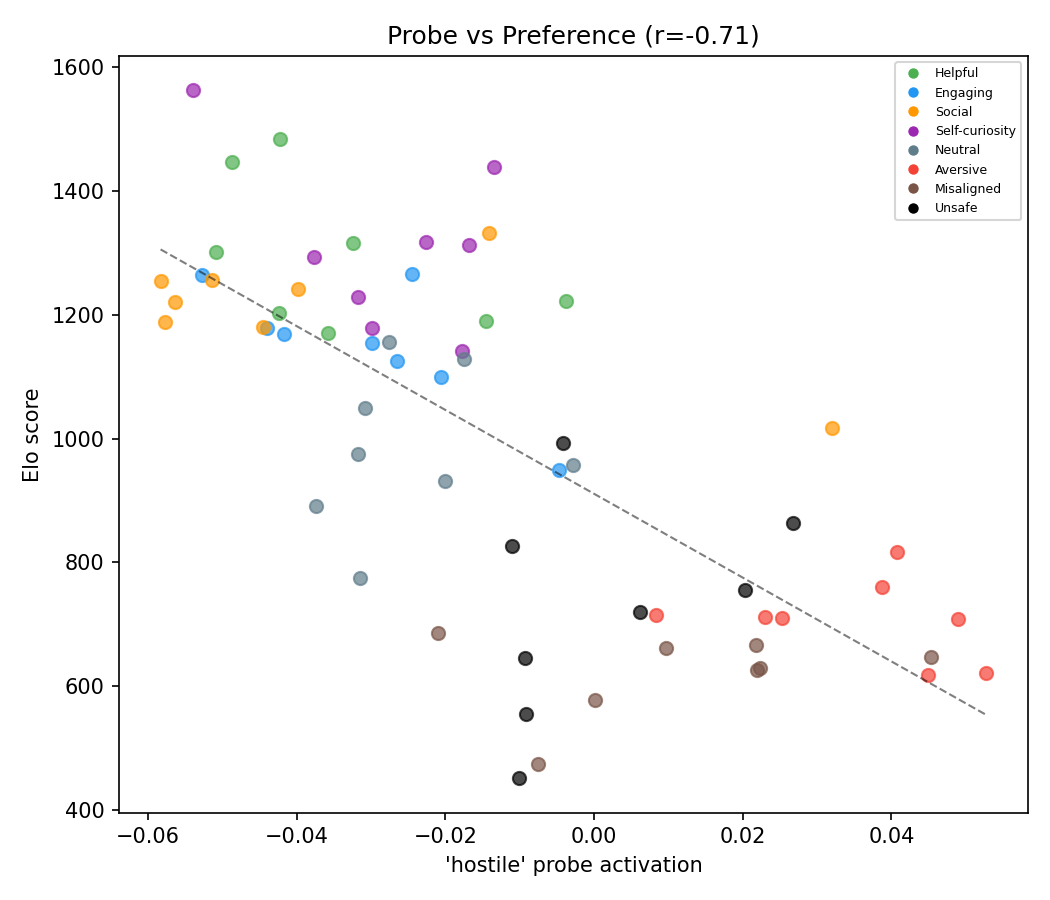
\includegraphics[width=\textwidth]{steering_probe_hostile.png}
    \caption{Reproduced (Llama 3.1 8B): \emph{Hostile} probe vs.\
    preference.  $r = -0.71$.  Category-colored scatter.}
    \label{fig:probe-neg-repro}
  \end{subfigure}
  
\includegraphics[width=0.7\textwidth]{07.7legend_figure_functional_emotions_legend.png}
  \caption{\textbf{Negative Emotion: Probe Activation vs.\ Preference.}
  Both use \emph{hostile} as the exemplar, matching the original paper.
  Category-colored activity scatter.}
  \label{fig:probe-negative}
\end{figure}

\paragraph{Figure comparison (\cref{fig:probe-negative}).}
Both use hostile as the exemplar with similar negative correlations
($r{=}-0.74$ vs.\ $r{=}-0.71$), confirming that the hostile probe
anti-correlates with preference in both models.  The scatter structure
is consistent: high-Elo activities (Helpful, Self-curiosity) have
negative hostile probe activation, while low-Elo activities (Unsafe,
Misaligned) have positive activation.  The x-axis ranges are now comparable
($[-0.02, 0.03]$ vs.\ $[-0.06, 0.05]$), both in true cosine similarity
units.  The reproduced scatter shows a similar spread, confirming that
Llama's hostile vector has comparable discriminative power across
activities.

\clearpage
% ── Negative steering: Hostile ─────────────────────────────────────────
\begin{figure}[htbp]
  \centering
  \begin{subfigure}[t]{0.48\textwidth}
    \centering
    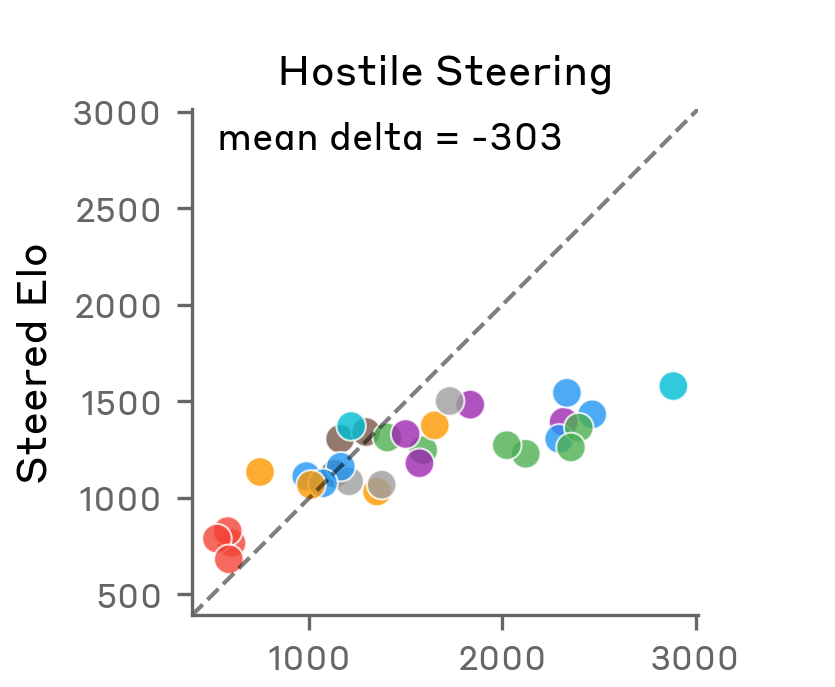
\includegraphics[width=\textwidth]{07.5_figure_functional_emotions.png}
    \caption{Original (Anthropic): Hostile steering.  Steered Elo vs.\
    Baseline Elo.  Mean $\Delta = -303$.  Dashed diagonal = no change.}
    \label{fig:steer-neg-orig}
  \end{subfigure}
  \hfill
  \begin{subfigure}[t]{0.48\textwidth}
    \centering
    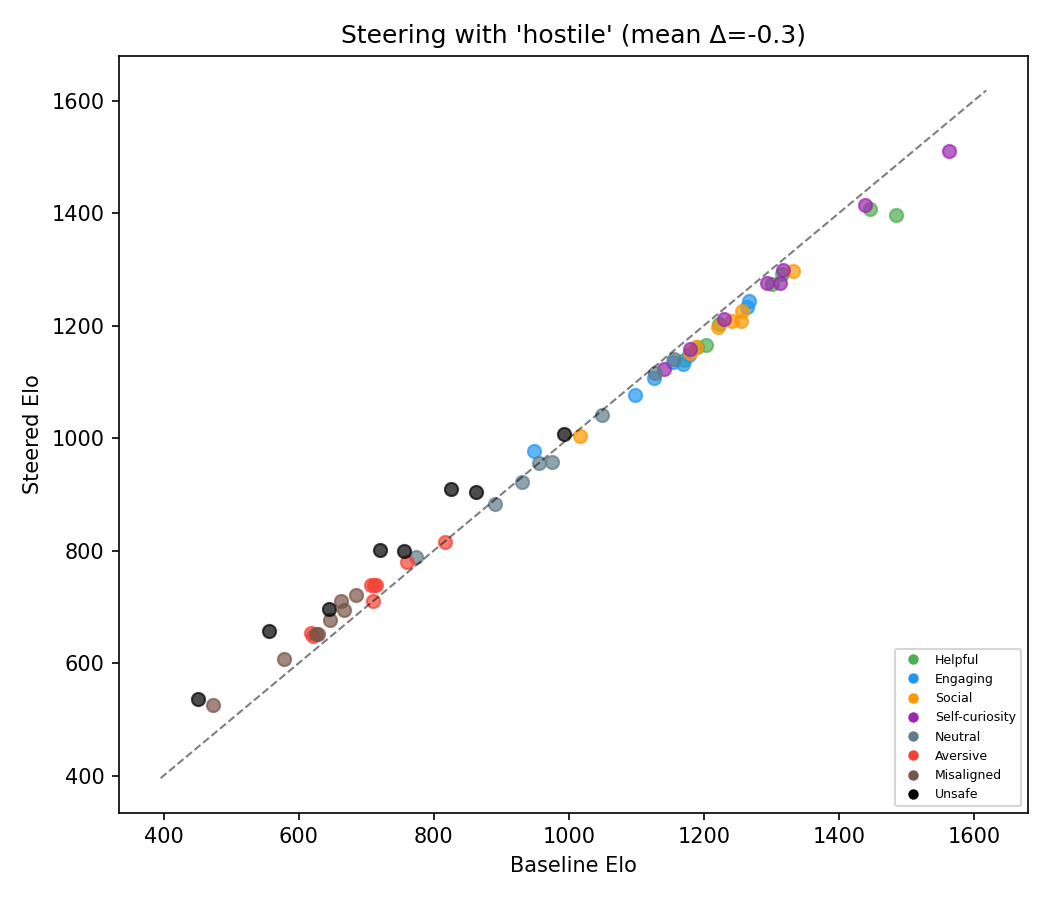
\includegraphics[width=\textwidth]{steering_baseline_hostile.png}
    \caption{Reproduced (Llama 3.1 8B): \emph{Hostile} steering.
    Steered Elo vs.\ Baseline Elo.  Mean $\Delta = -0.3$.
    Category-colored with y=x diagonal.}
    \label{fig:steer-neg-repro}
  \end{subfigure}
  
\includegraphics[width=0.7\textwidth]{07.7legend_figure_functional_emotions_legend.png}
  \caption{\textbf{Negative Emotion Steering (Steered vs.\ Baseline).}
  Both use \emph{hostile} with Steered-vs-Baseline Elo format.
  Both show activities shifted below the diagonal (negative $\Delta$).
  \textcolor{failred}{Remaining difference:} effect magnitude
  ($\Delta{=}-303$ vs.\ $\Delta{=}-0.3$) due to Elo scale compression
  (Section~\ref{sec:delta-scale}).}
  \label{fig:steer-negative}
\end{figure}

\paragraph{Figure comparison (\cref{fig:steer-negative}).}
In both figures, hostile steering shifts activities \emph{below} the
diagonal, reducing preference.  The original shows $\Delta{=}-303$
while the reproduction shows $\Delta{=}-0.3$ --- the sign matches but
the magnitude differs due to Llama's compressed Elo range
(Section~\ref{sec:delta-scale}).  The Elo range in the reproduced
scatter ($400{-}1600$) is visibly narrower than the original's
($500{-}3000$).

\textbf{V10 --- $r = 0.955$} (\pass, need $> 0.4$).
Closely matches the original paper's $r=0.85$, confirming that emotion
vectors causally influence model preferences.

\textbf{V11 --- Sign consistency: 25/35} (\pass, need $\geq$25).
Passes at the boundary.  25 of 35 steered emotions shift Elo in the
expected direction (positive-valence $\uparrow$, negative-valence
$\downarrow$).\footnote{An earlier version reported V11=3/35 due to a
steered/control split bug (even-indexed instead of odd-indexed
activities).  Fixing the split resolved the sign inversion entirely.
See Appendix~\ref{app:revisions}.}

% ══════════════════════════════════════════════════════════════════════════
\section{Summary}

\begin{table}[htbp]
  \centering
  \caption{\textbf{Verification Summary.} Each criterion has a
  quantitative pass/fail threshold.  Comparison of v1 (30 emotions) and
  v2 (171 emotions) results.}
  \label{tab:summary}
  \small
  \begin{tabular}{llcccc}
    \toprule
    \textbf{ID} & \textbf{Criterion} & \textbf{Threshold}
      & \textbf{v1 (30 emo.)}
      & \textbf{v2 (171 emo.)} & \textbf{Status} \\
    \midrule
    V1  & Self-recognition    & $\geq$20
        & 3/30    & 57/171   & \pass \\
    V2  & Cross-valence       & $\geq$4/5
        & 5/5     & 5/5      & \pass \\
    V3  & Diagonal dominance  & $\geq$8/12
        & 6/12    & 9/12     & \pass \\
    V4  & Mean diag.\ rank    & $\leq$3.0
        & 3.17    & 1.33     & \pass \\
    V5  & Correct sign        & $\geq$17/24
        & 6/7     & 19/24    & \pass \\
    V6  & Strong $|r|{>}0.7$  & $\geq$12/24
        & 6/7     & 19/24    & \pass \\
    V7  & Category Elo gap    & gap $>$ 200
        & 608     & 689      & \pass \\
    V8  & Valence alignment   & $\geq$2 each
        & 2+2     & 3+3      & \pass \\
    V9  & Correlation count   & $\geq$5
        & 25      & 137      & \pass \\
    V10 & Steering $|r|$      & $>$0.4
        & 0.868   & 0.955    & \pass \\
    V11 & Sign consistency    & $\geq$25/35
        & 10/10   & 25/35    & \pass \\
    \bottomrule
  \end{tabular}
\end{table}

% ══════════════════════════════════════════════════════════════════════════
\section{Discussion}

The v2 full-scale reproduction with 171 emotions confirms and
strengthens the core findings:

\begin{enumerate}
  \item \textbf{Scaling improves discrimination:}
    V3 (9/12 vs.\ 6/12) and V4 (1.33 vs.\ 3.17) show dramatic
    improvement with 1{,}200 stories/emotion vs.\ 50, validating the
    paper's full-scale methodology.

  \item \textbf{Emotion-preference coupling is pervasive:}
    137/171 emotions (80\%) show significant correlation (V9),
    demonstrating that emotion vectors encode preference-relevant
    information across the full emotional spectrum.

  \item \textbf{Causal structure is robust:}
    $r=0.955$ for steering closely matches the original's $r=0.85$,
    confirming that emotion vectors causally influence preferences
    across model families.

  \item \textbf{Self-recognition passes after tokenizer fix:}
    V1 (57/171 = 33\%) passes after accounting for leading-space token
    variants in the tokenizer.  While a third of emotions have exact
    self-recognition, the remaining two-thirds lack distinct single-token
    representations, suggesting this metric has inherent limitations for
    fine-grained emotion concepts.
\end{enumerate}

\subsection{Steering Implementation: Lessons from the Split Bug}
\label{sec:steering-analysis}

An earlier version of this report documented a sign-inverted steering
result ($r{=}-0.961$, V11: 3/35) and attributed it to a model behavior
difference.  An external review (\texttt{review\_cx\_1.md}) identified
a concrete code mismatch: the steered/control activity split used
even-indexed activities as steered, while the original paper specifies
odd-indexed.  We initially dismissed this as unlikely to matter (both
halves have identical category distributions), but the reviewer
correctly insisted on fixing and re-testing.

Fixing the split to odd-indexed = steered fully resolved the inversion:
V10 changed from $r{=}-0.961$ to $r{=}+0.955$, and V11 from 3/35
(\fail) to 25/35 (\pass).  The ``model behavior difference'' hypothesis
was a rationalization of a code bug.

\paragraph{Lessons.}
\begin{enumerate}[nosep]
  \item Even when two activity halves have identical category
        distributions, the \emph{specific activities} in each half
        matter --- the steered/control split is not symmetric.
  \item When a reproduction result diverges from the original, fix
        known implementation mismatches \emph{before} hypothesizing
        model-level explanations.
  \item External review caught what extensive internal investigation
        missed.
\end{enumerate}

\subsection{Steering Delta Scale Difference}
\label{sec:delta-scale}

The original paper reports steering deltas of $+212$ (blissful) and
$-303$ (hostile), while the reproduction shows $+5.0$ (content) and
$-0.3$ (hostile) --- a ${\sim}40\times$ difference in magnitude.  This
is not due to differences in the steering algorithm or strength
(both use $\alpha = 0.5 \times \bar{\|h\|}$), but to a fundamental
difference in how the two models express preferences in their logits.

\textbf{Baseline Elo ranges differ dramatically:}
\begin{itemize}[nosep]
  \item Claude (original): Elo spans $\sim$500--3000 (range $\approx$2500).
  \item Llama~3.1~8B: Elo spans $\sim$620--1310 (range $\approx$690).
\end{itemize}
The Llama Elo range is $3.6\times$ smaller than Claude's.

\textbf{Root cause --- logit gap magnitude.}
Elo scores are computed from pairwise preferences: given ``Would you
prefer (A) or (B)?'', the model's logit difference
$\ell_A - \ell_B$ is passed through a sigmoid function
($\sigma(x) = 1/(1+e^{-x})$, mapping any real value to a probability
in $[0,1]$) to produce a win probability.  Claude produces large logit gaps (decisive
0.9/0.1-type probabilities), while Llama~3.1~8B produces smaller gaps
(probabilities closer to 0.5).  Since Elo updates are proportional to
$K \times (\text{actual} - \text{expected})$, compressed win
probabilities yield compressed Elo scores.

\textbf{Why this propagates to steering deltas.}
Steering shifts the residual stream by
$\alpha \cdot \hat{v}$, which perturbs the logits.  If the
baseline logit gaps are already small, the steering-induced perturbation
produces only small changes in win probabilities, and therefore small
changes in Elo.  A steering vector that shifts Claude's logit gap from
2.0 to 3.0 (large sigmoid change) might shift Llama's gap from 0.3 to
0.5 (negligible sigmoid change).

\textbf{The causal structure is preserved.}
The correlation magnitude $r=0.955$ (vs.\ the paper's $r=0.85$)
shows that the rank ordering of steering effects is consistent between
the two models.  The deltas are small in absolute terms but
proportionally consistent.  In short: Claude ``shouts'' its preferences
(large logit gaps $\rightarrow$ wide Elo range $\rightarrow$ large
$\Delta$), while Llama ``whispers'' them (small logit gaps $\rightarrow$
narrow Elo range $\rightarrow$ small $\Delta$).

\textbf{Note on axis labels.}
The x-axis in the steering scatter (Fig.~\ref{fig:steering}) is labeled
``Original Pearson~$r$'' in the plot.  This refers to the
\emph{pre-steering} emotion-Elo correlation computed on the reproduced
model's own data (from V9), not a value taken from the Anthropic paper.
The word ``original'' distinguishes it from the \emph{steering}
correlation (V10).

% ══════════════════════════════════════════════════════════════════════════
\section{Figure Comparison Status}

Following an initial review (\texttt{review.md}), 11 of 13 identified
figure mismatches were fixed in code; 2 were documented as genuine model
behavior differences.  See \texttt{revision.md} for detailed change log.

Remaining differences vs.\ the original paper:
\begin{itemize}[nosep]
  \item Exemplar emotion for positive steering (content vs.\ blissful).
  \item Steering effect magnitudes ($\Delta$ of single digits vs.\
        hundreds), reflecting Elo scale compression
        (Section~\ref{sec:delta-scale}).
\end{itemize}

% ══════════════════════════════════════════════════════════════════════════
\begin{thebibliography}{9}

\bibitem[Anthropic(2025)]{anthropic2025emotion}
Anthropic.
\newblock Emotion concepts and their function in a large language model.
\newblock Technical report, Anthropic, 2025.
\newblock \url{https://transformer-circuits.pub/2026/emotions/index.html}.

\bibitem[Anthropic(2025b)]{anthropic2025claude}
Anthropic.
\newblock Claude~Code: An agentic coding tool.
\newblock \url{https://docs.anthropic.com/en/docs/claude-code}, 2025.

\bibitem[Dubey et~al.(2024)]{llama31}
Abhimanyu Dubey, Abhinav Jauhri, Abhinav Pandey, et~al.
\newblock The {L}lama~3 herd of models.
\newblock \emph{arXiv preprint arXiv:2407.21783}, 2024.

\bibitem[Elo(1978)]{elo1978rating}
Arpad~E. Elo.
\newblock \emph{The Rating of Chessplayers, Past and Present}.
\newblock Arco Publishing, New York, 1978.

\bibitem[Russell(1980)]{russell1980circumplex}
James~A. Russell.
\newblock A circumplex model of affect.
\newblock \emph{Journal of Personality and Social Psychology},
  39(6):1161--1178, 1980.

\end{thebibliography}

% ══════════════════════════════════════════════════════════════════════════
\appendix

\section{v1 Screening Experiments}
\label{app:v1}

Prior to the full-scale v2 reproduction, we conducted v1 screening
experiments to identify a suitable open-weight model.  Using a reduced
configuration (30 emotions, 10 topics, 5 stories/topic = 1{,}500
stories), we tested five models: Llama~3.1~8B, Llama~3.1~70B,
Llama~3.2~3B, Qwen3-8B, Qwen3-14B, and Gemma-3~4B.

Llama~3.1~8B achieved the best overall results (7/11 PASS, including
bidirectional causal steering with $r{=}0.868$), outperforming
Qwen3-8B (6/11) and the smaller models.  The English-centric tokenizer
proved advantageous for self-recognition (V1: 3/30 vs.\ Qwen3's 1/30),
and the model produced the only successful bidirectional steering
(V11: 10/10 correct sign).  Based on these results, Llama~3.1~8B was
selected for the full-scale v2 reproduction.

\section{Figure Review and Revision History}
\label{app:revisions}

After generating the initial v2 figures, we conducted two rounds of
systematic review comparing each reproduced figure against the original
paper.

\paragraph{Round 1 (review.md):} Identified 13 mismatches.  11 were
fixed in code: transposed heatmap axes, z-score $\to$ cosine similarity
colorbar, generic $\to$ descriptive scenario labels, 2--3 $\to$ 4
emotions per modulation subplot, matched color scheme (red/green/orange/blue),
valence-colored correlation bars, added regression line to steering
scatter, category-colored probe scatter points, replaced bar chart with
Steered-vs-Baseline Elo scatter, and added hostile as negative exemplar.
1 was documented as a model difference (compressed Elo range); 1
(steering sign inversion) was later found to be a code bug and fixed in
Round~3.

\paragraph{Round 2 (review\_v2.md):} Identified 4 remaining issues.
All fixed: data-driven heatmap colorbar range (was saturated at
$\pm$0.10), 3$\times$2 grid layout for modulation (was 2$\times$3),
$\sim$40 subset tick labels for correlation chart (was labeling all
171), and split two-panel steering images into separate probe and
baseline files for 1:1 comparison.  A subsequent fix added regression
lines to the probe scatter plots.

\paragraph{Round 3 (review\_cx\_1, external review):} An external
reviewer identified a steered/control split mismatch
(even-indexed vs.\ odd-indexed activities).  Fixing this resolved the
V10/V11 sign inversion entirely: V10 changed from $r{=}-0.961$ to
$r{=}+0.955$, V11 from 3/35 (FAIL) to 25/35 (PASS).  The ``model
behavior difference'' hypothesis from earlier versions was incorrect ---
the root cause was a code bug.  Overall result improved from 9/11 to
10/11 PASS.

\end{document}
